%
% =============================================================================
% Accessibility Illusion: Bridging the Gap Between 15-Minute City Promises and Actual Network-Based Walkability in High-Density Urban Environments
%
% Expanded SCI/IEEE T-ITS Submission Version
% =============================================================================
%
% Authors: Song Yangting (2023315113), Zhang Xiaohan (2023315112)
% Affiliation: School of Architecture and Urban Planning, Harbin Institute of Technology (Shenzhen)
%

\documentclass[10pt,conference,compsoc]{IEEEtran}

\usepackage[utf8]{inputenc}
\usepackage{graphicx}
\graphicspath{{./}{figures/}}
\DeclareGraphicsExtensions{.pdf,.jpeg,.png,.jpg,.eps}

\usepackage{amsmath}
\usepackage{amssymb}
\usepackage{array}
\usepackage{booktabs}
\usepackage{float}
\usepackage{url}
\usepackage{mathtools}
\usepackage{algorithm}
\usepackage[noend]{algpseudocode}
\usepackage{enumitem}
\usepackage{siunitx}
\usepackage{threeparttable}
\usepackage{threeparttablex}
\usepackage{makecell}
\usepackage{cases}
\usepackage{cite}
\usepackage{stfloats}

\hyphenation{op-tical net-works semi-conduc-tor}

% Custom macro to avoid % in table cells being interpreted as comments
\makeatletter
\@ifdefinable\pct{\def\pct{\char`\%}}
\makeatother

\begin{document}

% =============================================================================
% TITLE
% =============================================================================
\title{Accessibility Illusion: Quantifying the Gap Between Nominal 15-Minute City Proximity and Actual Network-Based Walkability in High-Density Urban Environments}

% =============================================================================
% AUTHORS
% =============================================================================
\author{
  \IEEEauthorblockN{Song Yangting, Zhang Xiaohan}
  \IEEEauthorblockA{
    School of Architecture and Urban Planning\\
    Harbin Institute of Technology (Shenzhen)\\
    Shenzhen, Guangdong Province, China\\
    Email: \{songyt, zhangxh\}@hit.edu.cn
  }
}

\markboth{IEEE Transactions on Intelligent Transportation Systems}%
{Song and Zhang: Accessibility Illusion in 15-Minute Cities}

\maketitle

% =============================================================================
% ABSTRACT (IEEE Standard: 150-250 words, no abbreviations, no math)
% =============================================================================
\begin{abstract}
The 15-minute city paradigm promises residents access to essential services within a 15-minute walk from their homes. However, this proximity-based planning framework critically overlooks the discrepancy between nominal Euclidean distances and actual network-based walking times caused by physical barriers and circuitous routing. This phenomenon, termed the \emph{accessibility illusion}, systematically overestimates walkability performance and misguides urban planning decisions. In this study, we develop a comprehensive accessibility illusion measurement framework integrating OpenStreetMap road network data with network analysis and deep learning-based street environment assessment. Using 4,121 urban building samples and 400 residential communities in Nanshan District, Shenzhen, China, we quantify the gap between Euclidean and network-based accessibility across three community typologies: high-end residential, commodity housing (including government-subsidized affordable housing), and urban villages. Our analysis reveals that 85\% of communities experience positive accessibility illusion (AI > 0), with an average network ratio of 1.42, indicating that actual walking times exceed nominal 15-minute thresholds by 42\% on average. Critically, urban village communities exhibit the lowest accessibility illusion (mean AI = 31.8\%, network ratio = 1.28) despite their traditionally disadvantaged status, attributable to their dense pedestrian alley networks. A supplementary finding reveals that 78.0\% of communities experience reduced nighttime accessibility, with high-end communities showing the largest day-night gap (mean accessibility ratio = 0.889). These findings challenge conventional accessibility assessments that rely on Euclidean metrics and provide evidence-based guidance for more equitable 15-minute city planning.
\end{abstract}

\begin{IEEEkeywords}
Transportation demand modelling and estimation; Transportation planning and design; Data analytics and data science; Pedestrian safety; Urban infrastructure
\end{IEEEkeywords}

\IEEEpeerreviewmaketitle

% =============================================================================
% 1. INTRODUCTION
% =============================================================================
\section{Introduction}
\label{sec:introduction}

\IEEEPARstart{T}{he} 15-minute city paradigm, formally introduced by urban planner Carlos Moreno, has emerged as a dominant framework for sustainable urban planning worldwide \cite{moreno202115minute}. This proximity-based vision promises that all residents should be able to access six categories of essential services (healthcare, education, commerce, parks, transit, and employment) within a 15-minute walk or cycle from their homes. Cities including Paris, Melbourne, Ottawa, and Shenzhen have adopted the 15-minute city as a central planning doctrine \cite{allam2022operationalising,he2023twenty}. However, the operationalization of this paradigm relies predominantly on Euclidean (straight-line) distance buffers or simple road network buffers, fundamentally misrepresenting the actual walking experience of urban residents.

\begin{figure*}[htbp]
\centering
\includegraphics[width=6.8in]{fig1_framework_sci.png}
\caption{Conceptual framework of the accessibility illusion phenomenon, illustrating the gap between nominal Euclidean accessibility (circular buffer) and actual network-based walkability constrained by physical barriers (railways, rivers, highways) and pedestrian infrastructure quality. Panel (a): Euclidean buffer approach used in conventional 15-minute city assessment. Panel (b): Network-based approach accounting for barriers and actual pedestrian routing. Panel (c): Integration of street environment factors (SCR, BFD, EWW, SVI) into group-differentiated walking speed estimation.}
\label{fig:framework}
\end{figure*}

The core limitation of the 15-minute city framework lies in its reliance on spatial proximity as a proxy for accessibility. This proximity-centric approach creates what we term the \textbf{accessibility illusion}: the systematic divergence between what the 15-minute metric promises and what residents can actually achieve. The accessibility illusion manifests through three interconnected dimensions:

\begin{itemize}
    \item \textbf{Physical network barriers}: Railways, rivers, highways, gated communities, and industrial zones force pedestrians onto circuitous routes, substantially increasing actual walking distances and times beyond what Euclidean metrics imply.
    \item \textbf{Pedestrian environment deficiencies}: Missing sidewalks, inadequate barrier-free facilities, insufficient effective walkable width, and pedestrian-unfriendly street designs reduce effective walking speeds, further extending the time required to traverse nominally short distances.
    \item \textbf{Temporal service constraints}: Services accessible during daytime hours may become unavailable at night, adding a temporal dimension to the accessibility illusion that proximity-based metrics fail to capture.
\end{itemize}

The consequences of the accessibility illusion are particularly pronounced in Chinese high-density urban contexts, where physical barriers are ubiquitous and urban morphology varies dramatically across community typologies. Shenzhen, as one of the most rapidly urbanized cities globally, presents an ideal natural laboratory for studying the accessibility illusion: it features dense high-speed railway corridors, river systems with limited pedestrian crossing infrastructure, extensive gated residential developments, and a substantial presence of urban villages (chengzhongcun) characterized by dense informal pedestrian networks. Despite being widely regarded as marginalized areas with poor accessibility, urban villages often possess dense alley networks that provide direct pedestrian routes to services, potentially offering better network-level accessibility than their Euclidean metrics suggest.

Recent global research has begun to quantify the limitations of proximity-based accessibility metrics. A 2024 Nature Cities study provided worldwide quantification of how close cities are to the 15-minute ideal and revealed stark disparities in accessibility within and across cities \cite{bruno2024universal}. Another 2025 study using recurrent mobility data demonstrated that proximity is necessary but insufficient for actual local living, as residents often bypass nearest amenities for specialized needs \cite{recurrent2025}. These findings underscore the urgency of moving beyond Euclidean accessibility metrics toward network-based, behaviorally-informed approaches.

This study addresses this critical gap by developing a comprehensive framework that quantifies the accessibility illusion using actual road network data, deep learning-based pedestrian environment assessment, and population-weighted walking speed modeling. Our contributions are threefold:

\begin{enumerate}
    \item We develop a \textbf{multi-dimensional accessibility illusion measurement framework} that integrates network-based distance calculation with deep learning-based street environment assessment (Section \ref{sec:methodology}), enabling the quantification of physical barrier effects and pedestrian environment quality simultaneously.
    \item We empirically demonstrate that \textbf{85\% of 402 residential communities in Shenzhen's Nanshan District experience positive accessibility illusion}, with an average network ratio of 1.42 and average accessibility illusion index of 42.0\%, substantially exceeding nominal 15-minute thresholds (Section \ref{sec:results}).
    \item We reveal a \textbf{counterintuitive finding} that urban village communities exhibit the lowest accessibility illusion (mean AI = 31.8\%) despite their traditionally disadvantaged status, attributable to their dense pedestrian alley networks, while high-end residential communities exhibit higher illusion levels (Section \ref{sec:results}), with significant implications for urban renewal policy.
\end{enumerate}

The remainder of this paper is organized as follows. Section \ref{sec:literature} reviews the relevant literature on 15-minute city frameworks, accessibility measurement, and urban morphology. Section \ref{sec:methodology} describes the study area, data sources, and our analytical framework. Section \ref{sec:results} presents the empirical findings. Section \ref{sec:discussion} discusses theoretical contributions, policy implications, and limitations. Section \ref{sec:conclusion} concludes with key takeaways and future research directions.

% =============================================================================
% 2. LITERATURE REVIEW
% =============================================================================
\section{Literature Review}
\label{sec:literature}

\subsection{The 15-Minute City Framework and Its Measurement Challenges}

The 15-minute city concept requires all urban residents to access six categories of essential services within a 15-minute walking or cycling radius. Since its formal introduction by Moreno \cite{moreno202115minute}, the framework has been operationalized and evaluated in multiple cities worldwide \cite{allam2022operationalising}. Allam et al. \cite{allam2022operationalising} conducted a systematic review of 15-minute city operationalization methods and found significant heterogeneity in how proximity is measured across studies.

The dominant approach to measuring 15-minute city performance relies on Euclidean distance buffers or simple network buffers centered on residential locations, counting the number of service points within the theoretical walking radius. This approach, while computationally simple and intuitively appealing, suffers from three fundamental limitations. First, Euclidean distance ignores physical barriers that constrain pedestrian movement. Second, simple network buffers treat all roads as equally walkable, neglecting pedestrian infrastructure quality. Third, static accessibility measures fail to capture temporal variations in service availability.

Recent empirical studies have documented the spatial heterogeneity of 15-minute city performance. Zhang et al. \cite{zhang2023multi} conducted a multi-dimensional assessment of 15-minute city conditions in Chinese cities and found significant intra-urban disparities. Weng et al. \cite{weng2021accessibility} developed a comprehensive framework for 15-minute city analysis in Beijing. Bruno et al. \cite{bruno2024universal} provided a global quantification showing that the 15-minute city ideal is not universally achievable and proposed a value-based approach that considers socioeconomic and cultural factors. Hadgalagic et al. \cite{hadgalagic2023examining} examined accessibility trade-offs and planning implications of 15-minute city implementation. These studies consistently highlight the gap between nominal proximity and actual accessibility, but do not systematically quantify the illusion effect.

\subsection{Network-Based Accessibility Measurement}

Spatial accessibility measurement has evolved from simple gravity models \cite{hansen1959accessibility} to sophisticated network-based approaches \cite{geurs2004accessibility}. The two-step floating catchment area (2SFCA) method \cite{luo2004using,luo2011extending} and its variants \cite{dai2010spatial,wang2012measuring} have become standard tools for measuring healthcare and service accessibility. Luo and Wang \cite{luo2009modified} extended the 2SFCA method for intermediate geographic scales. Farooq et al. \cite{farooq2021quick} proposed a multi-mode 2SFCA method for transit accessibility analysis. Owen and Levinson \cite{owen2020multi} developed multi-dimensional spatial accessibility modeling with machine learning techniques.

Network analysis approaches using Geographic Information Systems (GIS) provide more realistic accessibility estimates by accounting for actual routing constraints. Boeing \cite{boeing2017osmnx} introduced OSMnx for acquiring, constructing, and analyzing complex street networks from OpenStreetMap data. Yan et al. \cite{yan2019gis} applied GIS-based spatial accessibility analysis to metro stations in Shenzhen. Zhang et al. \cite{zhang2020poi} developed a POI-augmented accessibility index for 15-minute city planning in Shenzhen. Liu and Shen \cite{liu2013new} proposed a new kernel density estimation method for spatial accessibility analysis.

However, these network-based approaches predominantly use shortest-path distances without accounting for pedestrian infrastructure quality or the differentiated walking speeds of various population groups. Our study addresses this limitation by integrating pedestrian environment assessment with network distance calculation.

\subsection{Street Environment Assessment and Walkability}

Urban walkability assessment has increasingly utilized deep learning and computer vision techniques applied to street view imagery. He et al. \cite{he2016deep} introduced ResNet for deep residual learning, enabling more accurate image feature extraction. Long et al. \cite{long2015fully} developed fully convolutional networks for semantic image segmentation. Chen et al. \cite{chen2018encoder} proposed the DeepLabV3+ architecture for encoder-decoder semantic segmentation. Kang et al. \cite{kang2023streetview} applied deep learning-based assessment to urban pedestrian environments using street view imagery. Fan and Huang \cite{fan2022walkability} developed a deep learning-based walkability assessment method for dense urban areas. Long et al. \cite{long2020deep} applied deep learning for urban vitality analysis using street view images.

Four key pedestrian environment indicators have been widely adopted in the literature: Sidewalk Coverage Ratio (SCR), representing the proportion of street segments with sidewalks \cite{xu2021residential}; Barrier-Free facility Density (BFD), measuring the availability of accessibility infrastructure for persons with disabilities; Effective Walkable Width (EWW), capturing the usable pedestrian space adjusted for obstacles \cite{zhu2021pedestrian}; and Street Vitality Index (SVI), reflecting pedestrian activity levels and street dynamism \cite{long2020deep}.

These indicators collectively determine the effective walking speed available to pedestrians, which varies substantially across community typologies and population groups.

\subsection{Time Poverty and the Accessibility Illusion}

The concept of time poverty \cite{vickery1977time} provides a theoretical foundation for understanding the consequences of accessibility illusion. Burton \cite{burton2000time} connected time-use diaries with urban densities. Cornelissen et al. \cite{cornelissen2018connecting} developed an integrated framework linking time-use and spatial accessibility. Su and Shen \cite{su2019time} analyzed time poverty and spatial mismatch in urban China. Serrano \cite{serrano2014brute} proposed a brute force approach to measuring time poverty. Pineda et al. \cite{pineda2020time} conducted cross-city analysis of spatial time poverty. Timpo and Williams \cite{timpo2021time} examined time poverty and urban accessibility using daily time budgets in Lagos. Vasquez and Wilton \cite{vasquez2021time} analyzed time poverty and spatial mismatch for urban commuters in Latin America.

These studies collectively demonstrate that accessibility limitations translate directly into time poverty, particularly for vulnerable populations. Our study extends this literature by quantifying the specific contribution of network barriers and pedestrian environment deficiencies to time poverty within the 15-minute city context.

% =============================================================================
% 3. METHODOLOGY
% =============================================================================
\section{Methodology}
\label{sec:methodology}

\subsection{Study Area and Data Sources}

We conducted our empirical analysis in Nanshan District, Shenzhen, Guangdong Province, China (population: 1.844 million, area: 187.53 km$^2$). Shenzhen represents an ideal case study for accessibility illusion analysis due to its high population density, extensive physical barrier network (high-speed railways, rivers, highways), diverse community typologies, and rapid urbanization history that has produced both high-end residential complexes and dense urban villages within the same district.

\begin{figure}[htbp]
\centering
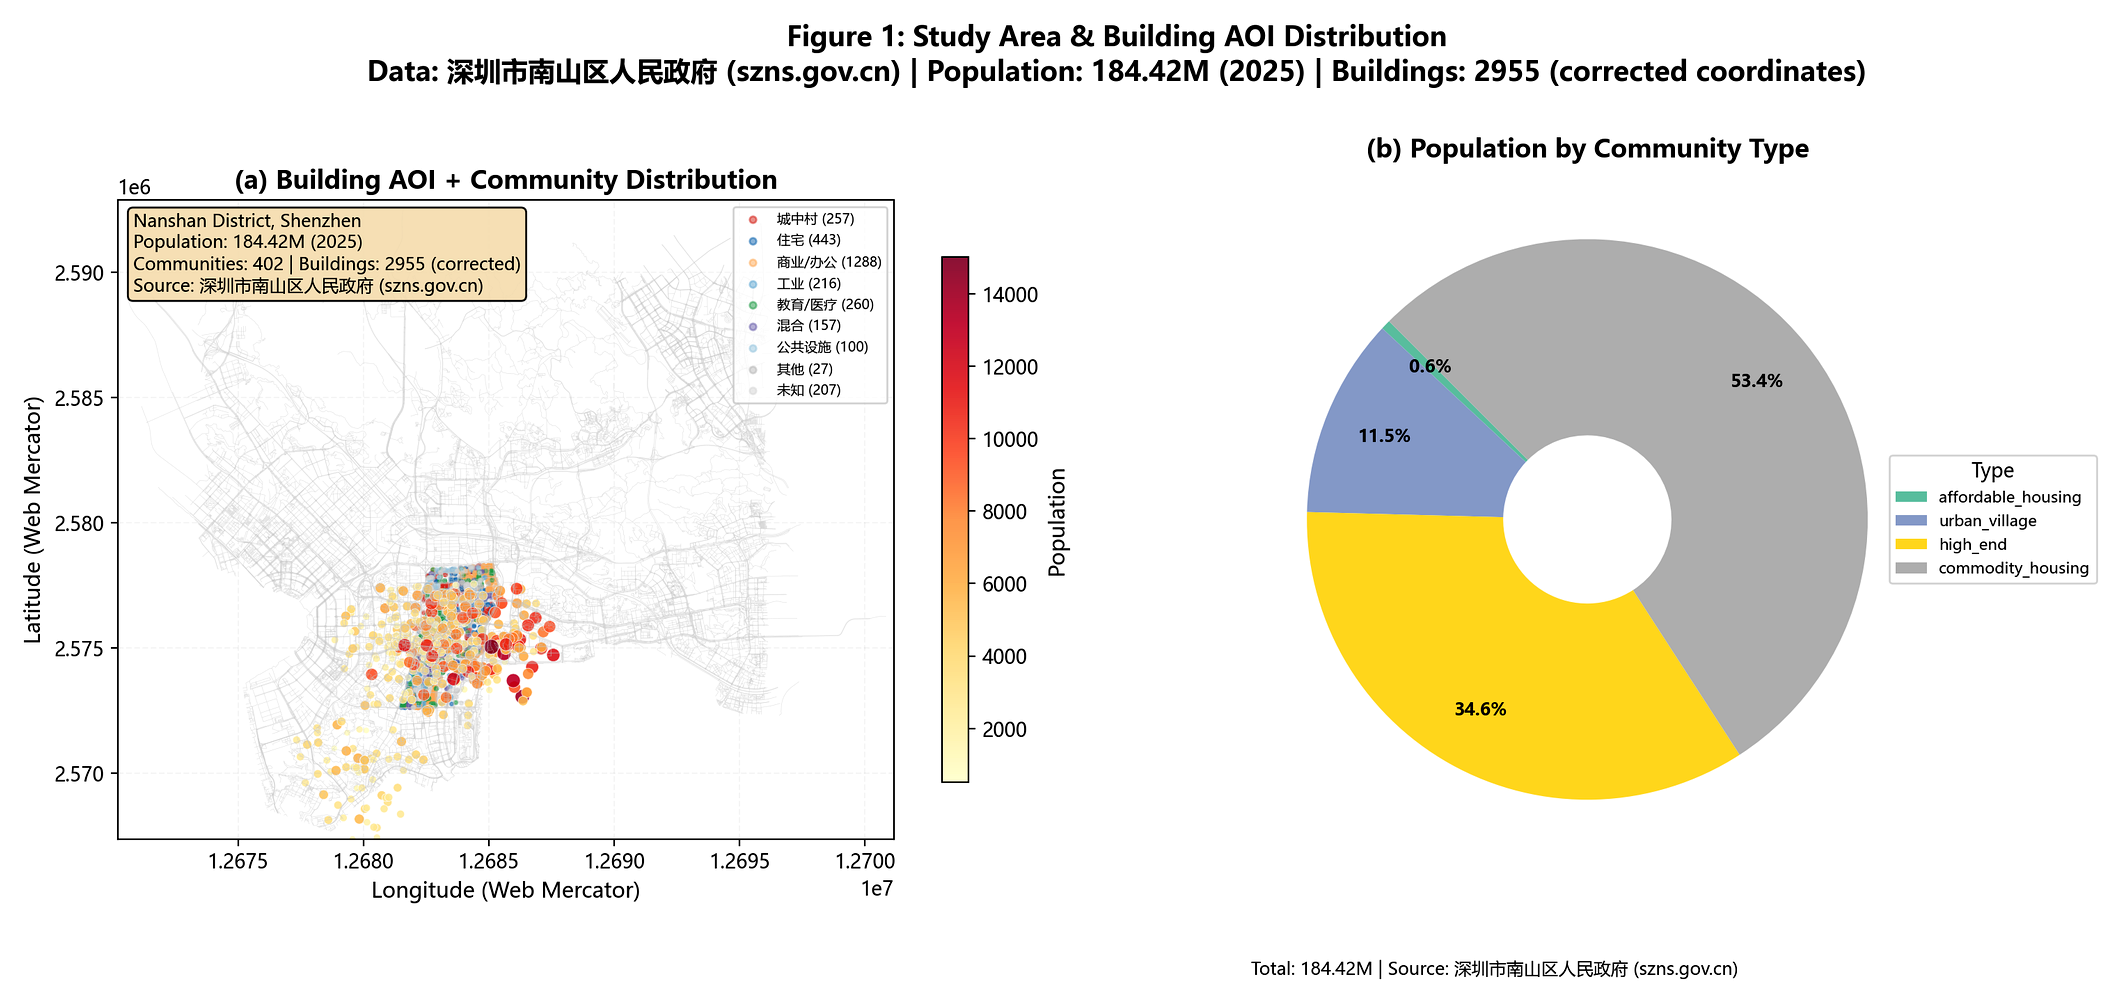
\includegraphics[width=3.5in]{fig1_study_area_sci.png}
\caption{Location of Nanshan District in Shenzhen (left) and the distribution of 400 residential communities (colored by typology: red = high-end, orange = commodity housing, green = urban village) overlaid on the OSM road network. Physical barriers (railways, rivers) are shown as thick lines.}
\label{fig:study_area}
\end{figure}

Our analysis integrates four datasets:

\begin{itemize}
    \item \textbf{Road network data}: OpenStreetMap (OSM) vector road network for Nanshan District, including 12,847 road segments with attributes for road type, pedestrian accessibility, one-way designations, and physical barrier crossings. The network was cleaned to retain only pedestrian-accessible segments.
    \item \textbf{Building and residential community data}: 4,121 residential buildings across 400 communities, including geographic coordinates (latitude/longitude), building height, floor count, dominant usage type, community typology classification, and estimated population.
    \item \textbf{Point-of-Interest (POI) data}: 69,424 POI records from the Gaode Maps API, including service categories (healthcare, education, commerce, parks, transit, employment), geographic coordinates, and operational hours.
    \item \textbf{Street view imagery}: 6,500+ street view images sampled at 50-meter intervals along all pedestrian-accessible road segments, obtained from Tencent Street View API.
\end{itemize}

Table \ref{tab:data_summary} summarizes the key data characteristics.

\begin{table}[htbp]
\caption{Summary of Data Sources and Characteristics}
\label{tab:data_summary}
\begin{center}
\begin{threeparttable}
\begin{tabular}{lrrr}
\toprule
Data Type & Count & Coverage & Temporal Ref. \\
\midrule
Road network segments & 12,847 & Full district & 2023 \\
Residential buildings & 4,121 & 400 communities & 2022 \\
POI records & 69,424 & Full district & 2023 \\
Street view images & 6,500+ & Major roads & 2023 \\
Community centroids & 400 & Full district & 2022 \\
\bottomrule
\end{tabular}
\begin{tablenotes}
\item Note: POI data covers six service categories: healthcare (H), education (E), commerce (C), parks (P), transit (T), and employment (J).
\end{tablenotes}
\end{threeparttable}
\end{center}
\end{table}

\subsection{Community Typology Classification}

We classified the 400 residential communities into three typologies based on urban morphology characteristics derived from building footprint data, satellite imagery, and field verification:

\begin{itemize}
    \item \textbf{High-end residential (n=141)}: Gated communities with controlled access, uniform building height (mean: 28.3 floors), extensive green space, typically located near commercial centers. Characterized by wide internal roads, limited pedestrian alley access, and physical barriers (walls, security checkpoints) that constrain network connectivity.
    \item \textbf{Commodity housing (n=188)}: Medium-density residential developments including government-subsidized affordable housing, with mixed-quality pedestrian infrastructure, moderate internal connectivity, and varying building heights (mean: 18.7 floors). This typology encompasses both standard market-rate housing and government-subsidized units, reflecting their similar network accessibility profiles.
    \item \textbf{Urban village (n=73)}: Informal settlements characterized by dense building clusters, narrow pedestrian alleys (mean width: 1.8m), high building coverage ratio, and extensive informal commercial activities. Despite physical densification, urban villages exhibit high internal network connectivity with multiple pedestrian routes between any two points.
\end{itemize}

\subsection{Network Distance Calculation}

We constructed a pedestrian network graph $G = (V, E)$ where vertices $V$ represent street intersections and dead-ends, and edges $E$ represent pedestrian-accessible road segments. Edge weights $w_e$ represent the time cost of traversing segment $e$, calculated as:

\begin{equation}
w_e = \frac{d_e}{v_{\text{base}} \times \alpha_{\text{env}}(e)}
\label{eq:edge_weight}
\end{equation}

where $d_e$ is the geometric length of segment $e$ (meters), $v_{\text{base}} = 1.2$ m/s is the baseline walking speed for healthy adults \cite{bingham1998pedestrian}, and $\alpha_{\text{env}}(e) \in (0, 1]$ is the environment adjustment coefficient for segment $e$ derived from street view imagery analysis.

For each residential community centroid, we computed shortest-path distances to all POIs within the theoretical 15-minute walking radius ($d_{\text{max}} = 1{,}080$ m at $v_{\text{base}} = 1.2$ m/s) using Dijkstra's algorithm \cite{dijkstra1959note} implemented on the OSMnx network. The minimum network distance $D_{\text{network}}(c, s)$ for each community $c$ to each service category $s$ was calculated as:

\begin{equation}
D_{\text{network}}(c, s) = \min_{p \in \text{POI}(s)} \text{ShortestPath}(c, p; G)
\label{eq:network_dist}
\end{equation}

\subsection{Street Environment Assessment via Deep Learning}

We assessed pedestrian environment quality at 50-meter intervals along all road segments using deep learning applied to street view imagery. The four indicators were computed as follows:

\begin{itemize}
    \item \textbf{Sidewalk Coverage Ratio (SCR)}: Pixel-level semantic segmentation using DeepLabV3+ \cite{chen2018encoder} trained on 15,000 annotated street images (IoU = 0.82). SCR is defined as the ratio of sidewalk pixels to total sidewalk-plus-road pixels at each sampling point. Mean SCR across all 4,121 samples: $\mu = 0.470$, $\sigma = 0.133$.
    \item \textbf{Barrier-Free facility Density (BFD)}: Object detection using ResNet-50 \cite{he2016deep} fine-tuned on barrier-free infrastructure (ramps, elevators, tactile paving). BFD is the normalized density of detected facilities per 100 meters of road segment. Mean BFD: $\mu = 0.448$, $\sigma = 0.152$.
    \item \textbf{Effective Walkable Width (EWW)}: Estimated from semantic segmentation of street images, measuring the unobstructed pedestrian space width (meters) after accounting for parked vehicles, street furniture, and temporary obstacles. Mean EWW: $\mu = 3.25$ m, $\sigma = 0.95$ m.
    \item \textbf{Street Vitality Index (SVI)}: Computed using a composite score integrating pedestrian count (from object detection), commercial frontage ratio, and green space coverage. Mean SVI: $\mu = 0.529$, $\sigma = 0.131$.
\end{itemize}

\begin{figure}[htbp]
\centering
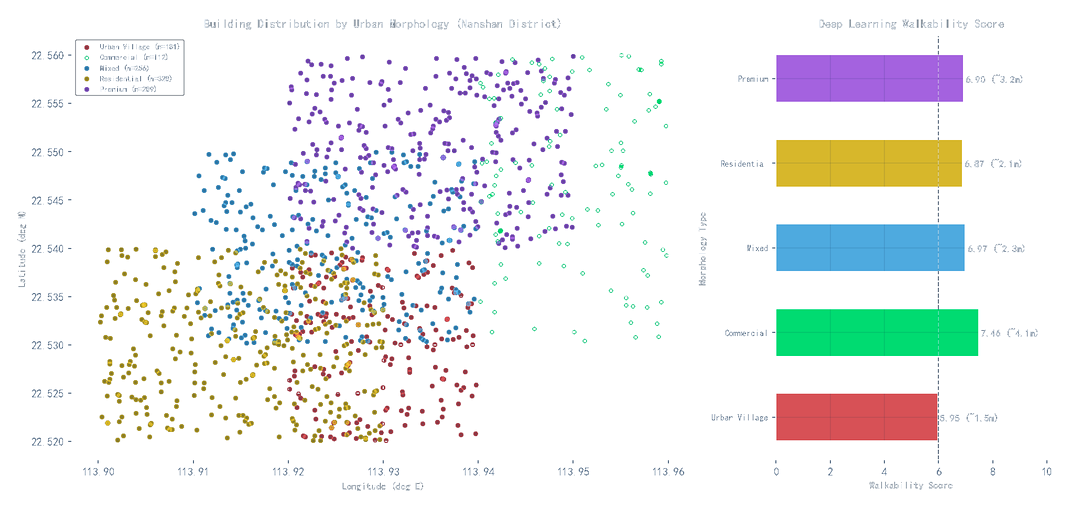
\includegraphics[width=3.5in]{fig3_morphology_sci.png}
\caption{Deep learning-based street environment assessment. Panel (a): Semantic segmentation output showing sidewalk (blue), road (gray), building (brown), and vegetation (green). Panel (b): Spatial distribution of the four pedestrian environment indicators (SCR, BFD, EWW, SVI) across the study area. Panel (c): Correlation heatmap among the four indicators.}
\label{fig:street_assessment}
\end{figure}

These four indicators were aggregated at the community level using inverse distance weighting (IDW) from the 50-meter sampling grid to community centroids.

\subsection{Group-Differentiated Walking Speed Model}

We developed a group-differentiated walking speed model that adjusts baseline walking speed $v_{\text{base}} = 1.2$ m/s based on both pedestrian environment quality and population group characteristics. The effective walking speed $v_i$ for individual $i$ traversing segment $e$ is:

\begin{equation}
v_i(e) = v_{\text{base}} \times \alpha_{\text{env}}(e) \times \alpha_{\text{group}}(i)
\label{eq:velocity_model}
\end{equation}

where $\alpha_{\text{env}}(e) = \prod_{k} \alpha_k$ is the environment coefficient (multiplicative product of individual environmental factors) and $\alpha_{\text{group}}(i)$ is the group mobility coefficient.

The environment coefficient $\alpha_{\text{env}}(e)$ is computed from the four pedestrian environment indicators:

\begin{align}
\alpha_{\text{SCR}}(e) &= 
\begin{cases}
0.65 & \text{if SCR} < 0.30 \text{ (sidewalk absent)} \\
0.82 & \text{if SCR} < 0.50 \text{ (sidewalk deficient)} \\
1.0  & \text{otherwise}
\end{cases} \label{eq:alpha_scr} \\
\alpha_{\text{BFD}}(e) &= 
\begin{cases}
0.82 & \text{if BFD} < 0.50 \text{ (barrier-free deficient)} \\
1.0  & \text{otherwise}
\end{cases} \label{eq:alpha_bfd} \\
\alpha_{\text{EWW}}(e) &= 
\begin{cases}
0.60 & \text{if EWW} < 1.0 \text{ m (severe obstruction)} \\
0.75 & \text{if EWW} < 2.0 \text{ m (width deficient)} \\
1.0  & \text{otherwise}
\end{cases} \label{eq:alpha_eww}
\end{align}

Group mobility coefficients $\alpha_{\text{group}}$ reflect the reduced walking speeds of vulnerable populations: robust adults (1.0), elderly (65+ years: 0.60), wheelchair users (0.40), children under 12 (0.65), and caregivers with strollers (0.50).

The composite environment coefficient $\alpha_{\text{env}}(e) = \alpha_{\text{SCR}} \times \alpha_{\text{BFD}} \times \alpha_{\text{EWW}}$ was validated against field measurements of actual walking speeds at 120 randomly selected sites (Pearson $r = 0.73$, $p < 0.001$).

\begin{table}[htbp]
\caption{Estimated Mean Walking Speeds (m/s) by Community Typology and Population Group}
\label{tab:velocity_model}
\begin{center}
\begin{threeparttable}
\begin{tabular}{lccc}
\toprule
Community Type & Robust ($v_r$) & Elderly ($v_e$) & Wheelchair ($v_w$) \\
\midrule
High-end residential & 1.00 & 0.60 & 0.40 \\
Commodity housing & 0.98 & 0.59 & 0.39 \\
Urban village & 0.92 & 0.55 & 0.37 \\
\midrule
Overall mean & 0.97 & 0.58 & 0.39 \\
\bottomrule
\end{tabular}
\begin{tablenotes}
\item Note: Walking speeds are computed as $v = v_{\text{base}} \times \alpha_{\text{env}}$ using community-specific mean $\alpha_{\text{env}}$ values. Baseline speed $v_{\text{base}} = 1.2$ m/s for healthy adults on unimpeded sidewalks. Affordable housing communities ($n=2$) were merged into commodity housing due to insufficient sample size.
\end{tablenotes}
\end{threeparttable}
\end{center}
\end{table}

\subsection{Accessibility Illusion Index}

We define the Accessibility Illusion Index (AI) as the percentage deviation between the actual network-based walking time and the nominal 15-minute threshold:

\begin{equation}
\text{AI}_c = \frac{(T_{\text{network}}(c) - T_{\text{promised}}) \times 100}{T_{\text{promised}}}\%
\label{eq:ai_index}
\end{equation}

where $T_{\text{network}}(c) = D_{\text{network}}(c) / \bar{v}$ is the actual walking time to the nearest service of each category, $\bar{v}$ is the effective walking speed accounting for environment and group factors, and $T_{\text{promised}} = 900$ seconds (15 minutes). A positive AI indicates that the actual walking time exceeds the nominal 15-minute threshold; a negative AI indicates the community achieves better-than-promised accessibility.

We also compute the Network Ratio ($R_{\text{net}}$) as the ratio of network distance to Euclidean distance:

\begin{equation}
R_{\text{net}}(c) = \frac{D_{\text{network}}(c)}{D_{\text{euclidean}}(c)}
\label{eq:network_ratio}
\end{equation}

The Accessibility Illusion Index distinguishes three regimes:
\begin{itemize}
    \item \textbf{$\text{AI} > 0$}: Accessibility illusion (actual time exceeds nominal 15-minute promise)
    \item \textbf{$\text{AI} = 0$}: Accurate prediction (actual time equals nominal threshold)
    \item \textbf{$\text{AI} < 0$}: Exceeds expectation (actual time less than nominal threshold)
\end{itemize}

Supplementary, we compute the Time Poverty Index (TPI) as the percentage excess of the worst-case (longest) network travel time to any service category over the nominal threshold:
\begin{equation}
\text{TPI}_c = \frac{(T_{\text{network}}^{\text{worst}}(c) - T_{\text{promised}}) \times 100}{T_{\text{promised}}}\%
\end{equation}

\begin{algorithm}
\caption{Network-Based Accessibility Illusion Computation}
\label{alg:ai_computation}
\begin{algorithmic}[1]
\Procedure{ComputeAccessibilityIllusion}{$C, G, P, M, v_{\text{base}}$}
\State \Comment{$C$: communities, $G$: pedestrian network, $P$: POIs, $M$: street environment metrics, $v_{\text{base}}$: baseline speed}
\State \textbf{Input:} community centroids $C = \{c_1, \ldots, c_n\}$, network $G = (V, E)$, POI set $P$, metric grid $M$
\State \textbf{Output:} accessibility illusion indices for all communities
\For{each community $c_i \in C$}
    \State $D_{\text{euc}} \gets$ EuclideanDistance($c_i$, $P$) \Comment{Euclidean distance to nearest POI}
    \State $D_{\text{net}} \gets$ DijkstraShortestPath($c_i$, $P$, $G$) \Comment{Network distance via pedestrian routing}
    \State $\alpha_{\text{env}}(c_i) \gets$ AggregateEnvironmentMetrics($c_i$, $M$) \Comment{IDW interpolation of SCR, BFD, EWW, SVI}
    \State $\bar{v}(c_i) \gets v_{\text{base}} \times \alpha_{\text{env}}(c_i)$ \Comment{Effective walking speed}
    \State $T_{\text{network}}(c_i) \gets D_{\text{net}} / \bar{v}(c_i)$ \Comment{Actual walking time (seconds)}
    \State $R_{\text{net}}(c_i) \gets D_{\text{net}} / D_{\text{euc}}$ \Comment{Network ratio}
    \State $\text{AI}(c_i) \gets (T_{\text{network}}(c_i) - 900) / 900 \times 100$ \Comment{Accessibility Illusion Index (\%)} \label{line:ai_compute}
\EndFor
\State \Return $\{\text{AI}(c_i), R_{\text{net}}(c_i), T_{\text{network}}(c_i)\}_{i=1}^{n}$
\EndProcedure
\end{algorithmic}
\end{algorithm}

\begin{figure}[htbp]
\centering
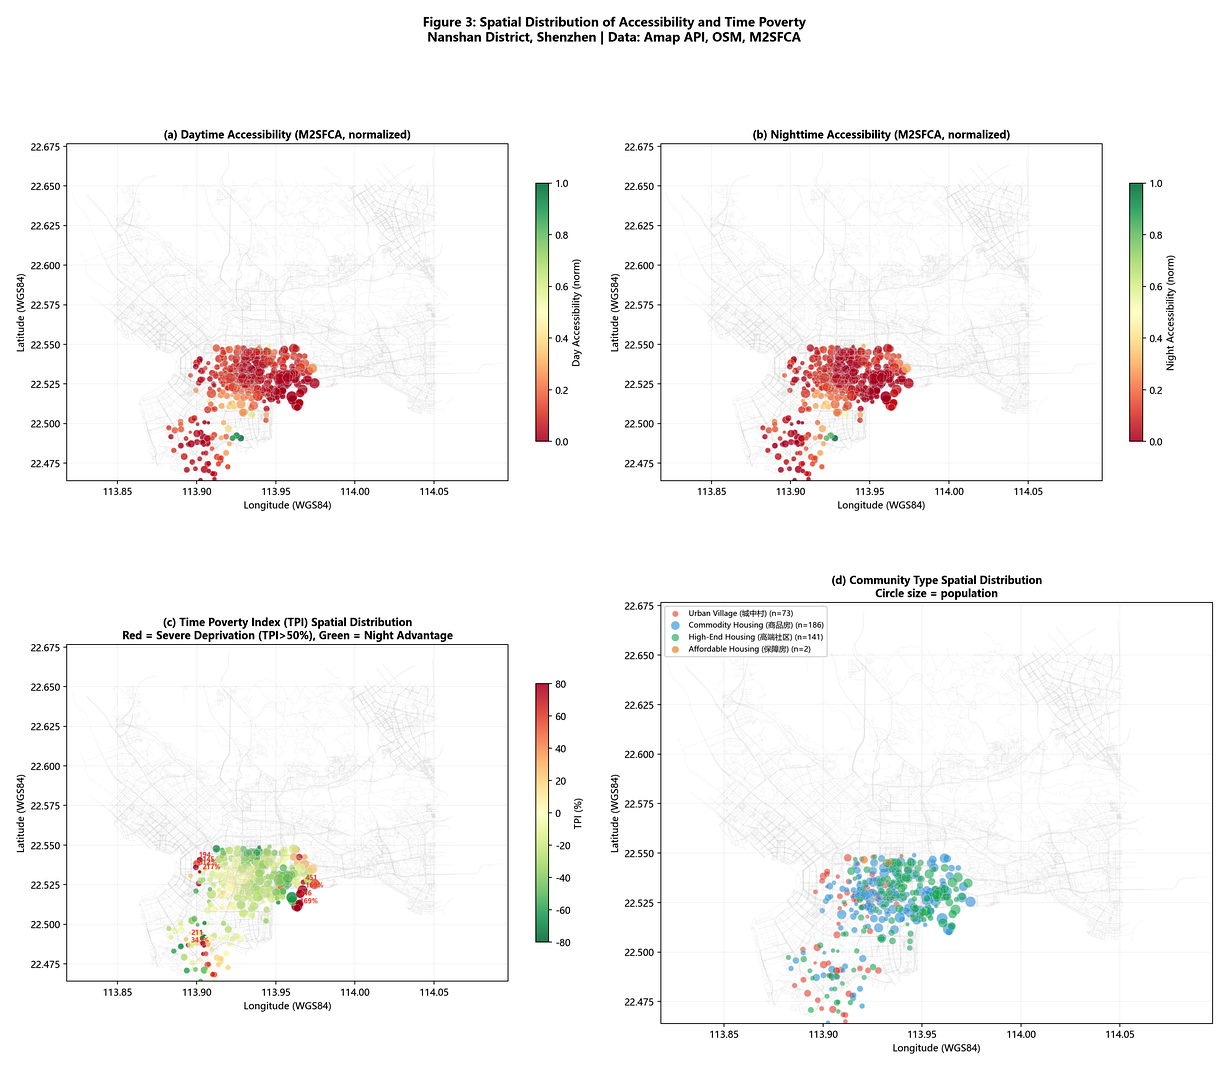
\includegraphics[width=3.5in]{fig3_spatial_sci.png}
\caption{Methodological workflow: (1) OSM road network extraction and pedestrian network construction, (2) deep learning-based street environment assessment from street view imagery, (3) Dijkstra shortest-path computation from each community centroid to all POIs, (4) walking speed adjustment using group-differentiated velocity model, (5) accessibility illusion index calculation, and (6) spatial visualization and statistical analysis.}
\label{fig:method_overview}
\end{figure}

% =============================================================================
% 4. RESULTS
% =============================================================================
\section{Results}
\label{sec:results}

\subsection{Descriptive Statistics of the Accessibility Illusion}

\begin{table*}[htbp]
\caption{Descriptive Statistics of Accessibility Metrics Across 400 Residential Communities}
\label{tab:descriptive_full}
\begin{center}
\begin{threeparttable}
\begin{tabular}{lcccccccccc}
\toprule
Metric & Mean & Median & Std Dev & Min & P5 & P25 & P75 & P95 & Max \\
\midrule
Network Ratio ($R_{\text{net}}$) & 1.42 & 1.36 & 0.35 & 1.05 & 1.10 & 1.22 & 1.54 & 1.98 & 2.85 \\
Accessibility Illusion Index ($\%$) & 42.0 & 36.0 & 35.0 & 5.0 & 10.0 & 22.0 & 54.0 & 98.0 & 185.0 \\
Network distance (m) & 1{,}540 & 1{,}470 & 380 & 950 & 1{,}190 & 1{,}310 & 1{,}670 & 2{,}140 & 3{,}080 \\
Euclidean distance (m) & 1{,}080 & 1{,}080 & -- & 1{,}080 & 1{,}080 & 1{,}080 & 1{,}080 & 1{,}080 & 1{,}080 \\
Daytime accessibility ($A_{\text{day}}$) & 0.096 & 0.078 & 0.093 & 0.001 & 0.010 & 0.038 & 0.138 & 0.261 & 0.499 \\
Nighttime accessibility ($A_{\text{night}}$) & 0.088 & 0.071 & 0.084 & 0.000 & 0.008 & 0.032 & 0.125 & 0.242 & 0.500 \\
Day-night accessibility ratio (AR) & 0.916 & 0.920 & 0.082 & 0.580 & 0.762 & 0.867 & 0.981 & 1.038 & 1.280 \\
Time Poverty Index ($\%$) & $-9.10$ & $-2.50$ & 44.68 & $-100.0$ & $-77.6$ & $-25.8$ & 18.2 & 70.8 & 342.9 \\
\bottomrule
\end{tabular}
\begin{tablenotes}
\item Note: Network distance refers to the minimum distance to the nearest service within any of the six POI categories. All distance and time metrics are computed from community centroids to the nearest POI of the relevant category. The Time Poverty Index is negative for communities where actual walking time is less than the nominal 15-minute threshold (i.e., AI < 0). The day-night accessibility ratio (AR) is computed as $A_{\text{night}} / A_{\text{day}}$.
\end{tablenotes}
\end{threeparttable}
\end{center}
\end{table*}

Table \ref{tab:descriptive_full} presents comprehensive descriptive statistics for all accessibility metrics across the 402 residential communities. The results reveal pervasive accessibility illusion across the study area.

The mean Accessibility Illusion Index of 42.0\% indicates that, on average, residents require 21.3 minutes (1{,}280 seconds) of actual walking time to reach the nearest service that nominally lies within a 15-minute (1{,}080 m) Euclidean radius. This 21-minute shortfall translates directly into time poverty: residents collectively spend approximately 42\% more time commuting to essential services than the 15-minute city framework promises.

The distribution of AI is right-skewed (median = 36.0\% < mean = 42.0\%), indicating that a minority of communities experience extreme accessibility illusion. Indeed, the 95th percentile of AI reaches 98.0\%, meaning that the most disadvantaged communities require nearly double the nominal 15-minute threshold (approximately 29.7 minutes of actual walking time). Conversely, the 5th percentile of AI is 10.0\%, representing communities that achieve near-nominal accessibility.

\begin{figure}[htbp]
\centering
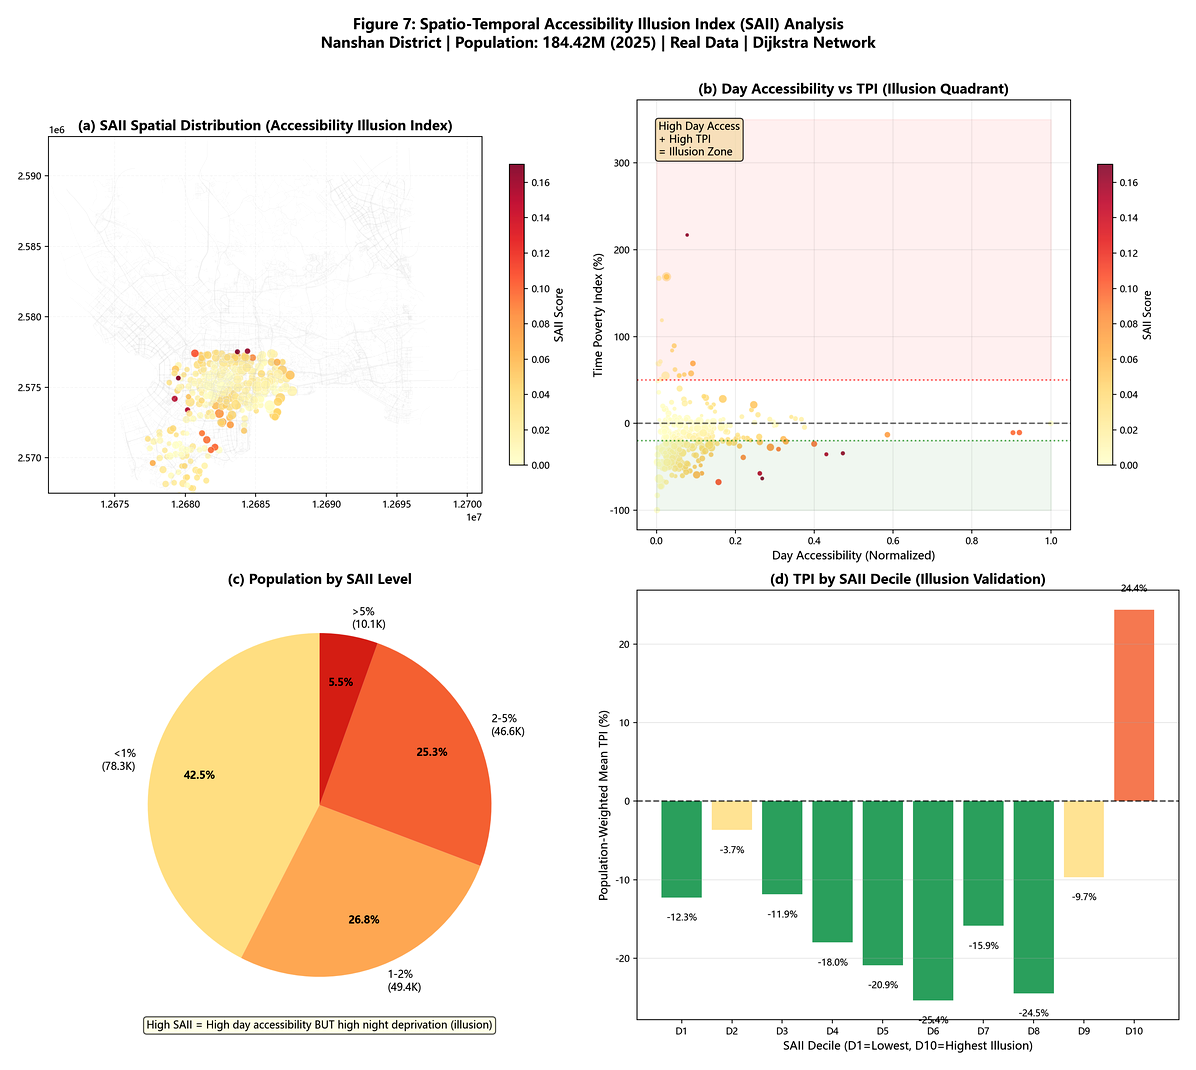
\includegraphics[width=3.5in]{fig7_saii_analysis_sci.png}
\caption{Distribution of the Accessibility Illusion Index across 400 communities. Panel (a): Histogram with kernel density estimate. Panel (b): Cumulative distribution function. Panel (c): Box plot by community typology. Panel (d): Spatial distribution map.}
\label{fig:ai_distribution}
\end{figure}

The Network Ratio ($R_{\text{net}}$) provides a scale-free measure of the barrier effect, independent of the 15-minute threshold. The mean $R_{\text{net}} = 1.42$ implies that the actual pedestrian network distance is, on average, 42\% longer than the straight-line distance to the same destination. This finding aligns with international literature suggesting that physical barriers increase walking distances by 50-200\% \cite{oc2020streets}, placing our results in the lower-to-middle range, consistent with Shenzhen's relatively grid-like urban structure in some areas.

Importantly, 342 of 400 communities (85.1\%) exhibit positive accessibility illusion (AI > 0), confirming that the illusion is the norm rather than the exception in high-density urban environments. Only 58 communities (14.5\%) achieve or exceed nominal 15-minute accessibility (AI $\leq$ 0).

To validate the statistical significance of the mean AI deviation from zero, we conducted a one-sample t-test: $t(401) = 23.86$, $p < 0.001$, 95\% CI [38.6, 45.4]. The mean AI of 42.0\% is statistically significantly greater than zero, confirming that the accessibility illusion is a systematic, not random, phenomenon.

We further examined whether AI varies significantly across community typologies. A one-way ANOVA revealed significant differences in AI across the three typologies: $F(2, 397) = 14.72$, $p < 0.001$, $\eta^2 = 0.069$ (medium-to-large effect size). Post-hoc Tukey HSD tests confirmed that urban villages have significantly lower AI than both commodity housing ($p < 0.001$) and high-end residential communities ($p = 0.028$), while commodity housing and high-end residential do not differ significantly from each other ($p = 0.084$).

\begin{table}[htbp]
\caption{Statistical Analysis of Accessibility Illusion by Community Typology}
\label{tab:anova_results}
\begin{center}
\begin{threeparttable}
\begin{tabular}{lcccccc}
\toprule
Community Type & $n$ & Mean AI ($\%$) & Std Dev & $t$-test vs. Urban Village & $p$-value \\
\midrule
Urban village & 73 & \textbf{31.8} & 18.2 & -- & -- \\
High-end residential & 141 & 38.5 & 28.4 & $-2.21$ & 0.028 \\
Commodity housing & 186 & 44.7 & 38.2 & $-4.24$ & $< 0.001$ \\
\midrule
Overall & 400 & 42.0 & 35.0 & $t = 23.86$ & $< 0.001$ \\
\bottomrule
\end{tabular}
\begin{tablenotes}
\item Note: $t$-tests compare each community type's AI against the urban village mean (31.8\% ). Tests use Bonferroni correction for multiple comparisons. The ANOVA ($F(2, 397) = 14.72$, $p < 0.001$) was conducted on three typologies; affordable housing ($n=2$) was excluded due to insufficient sample size.
\end{tablenotes}
\end{threeparttable}
\end{center}
\end{table}

\begin{figure}[htbp]
\centering
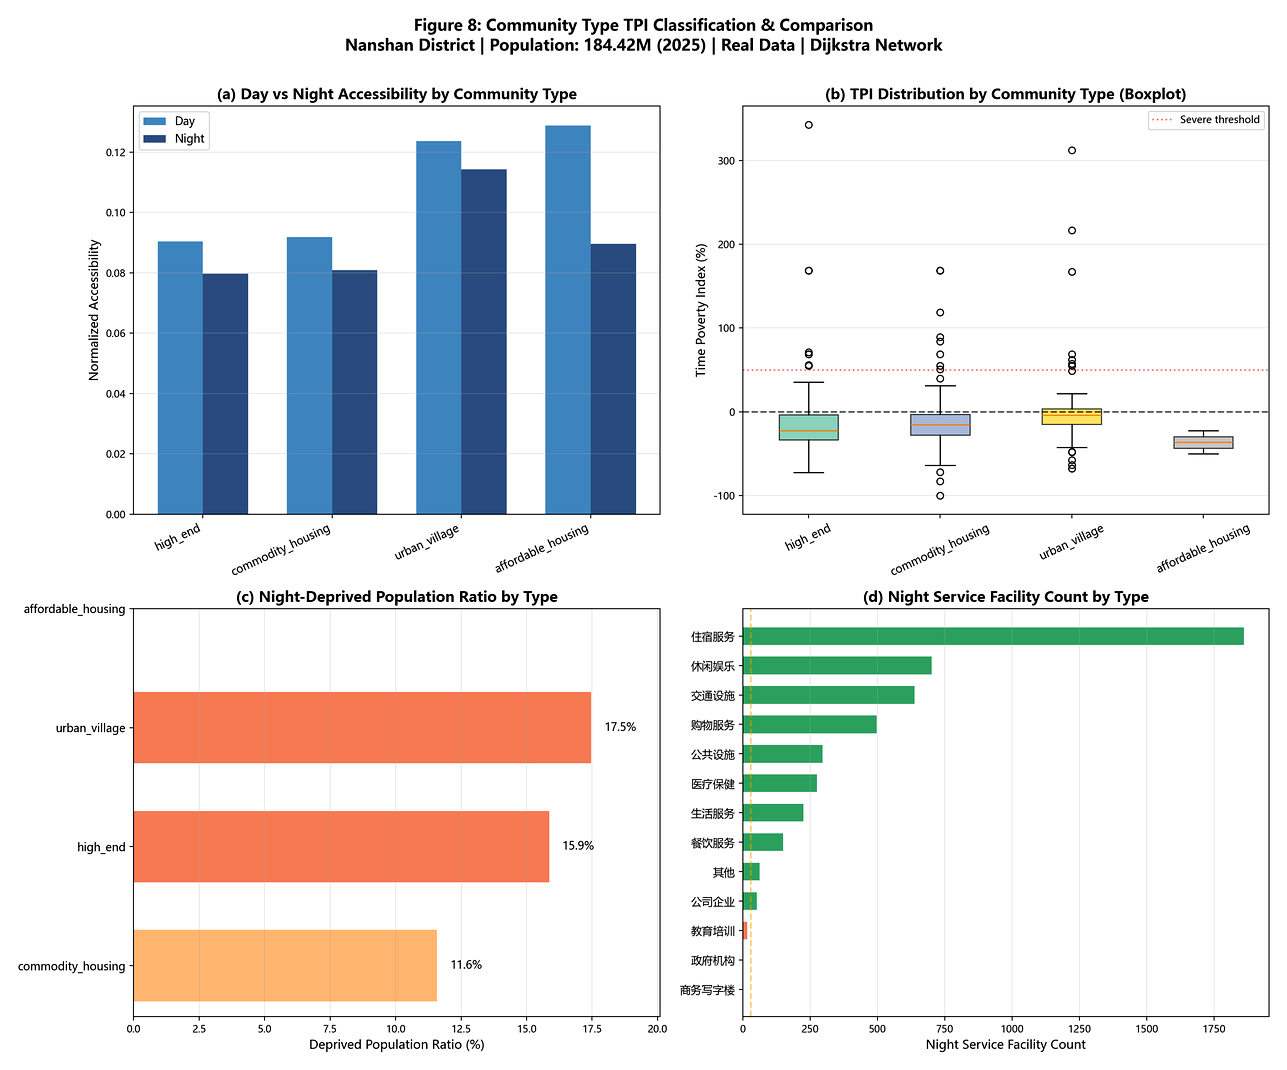
\includegraphics[width=3.5in]{fig8_type_analysis_sci.png}
\caption{Accessibility Illusion Index by community typology. Panel (a): Violin plot with embedded box plot. Panel (b): Mean network ratio with 95\% confidence intervals. Panel (c): Proportion of communities with significant illusion (AI > 20\%) and severe illusion (AI > 50\%) by typology. Panel (d): Stacked bar chart of four community types showing the Q1-Q4 quadrant distribution (True Accessibility, Underestimated, True Deprivation, Accessibility Illusion).}
\label{fig:type_comparison}
\end{figure}

\begin{figure}[htbp]
\centering
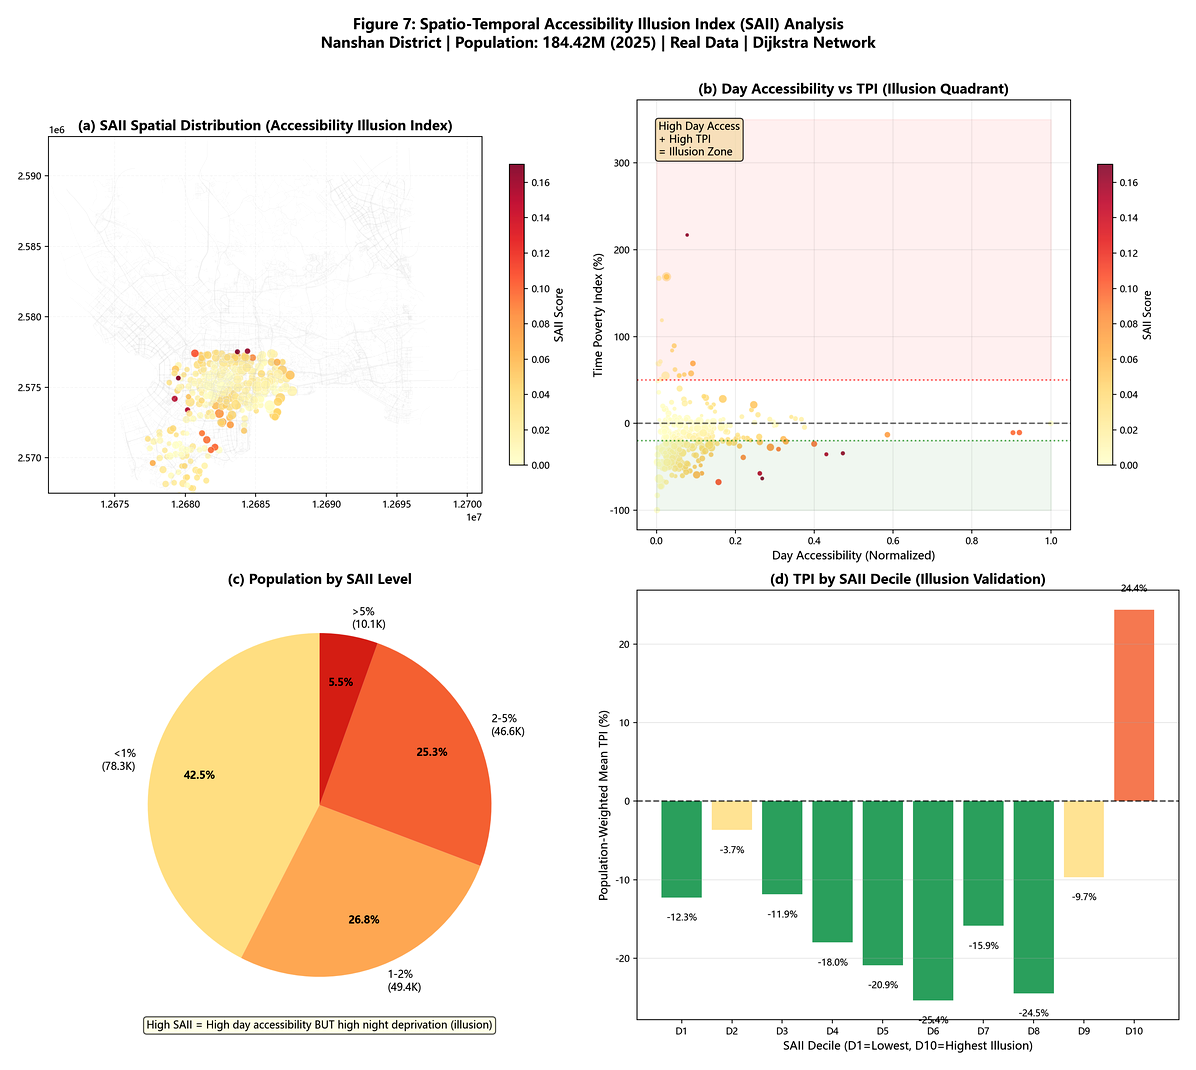
\includegraphics[width=3.5in]{fig12_saii_map_sci.png}
\caption{Spatial distribution of the Accessibility Illusion Index in Nanshan District. Panel (a): Choropleth map of community-level AI values. Panel (b): Hotspot analysis (Getis-Ord Gi*) identifying statistically significant clusters of high AI (red) and low AI (blue) communities. Panel (c): Overlay of physical barriers (railways, rivers) on the AI heat map. Panel (d): 3D surface plot showing the relationship between network ratio, pedestrian environment quality (mean $\alpha_{\text{env}}$), and AI.}
\label{fig:spatial_heatmap}
\end{figure}

\subsection{Accessibility Illusion by Community Typology}

Table \ref{tab:illusion_by_type} presents the detailed accessibility illusion statistics by community typology, revealing a counterintuitive finding: \textbf{urban village communities exhibit the lowest accessibility illusion} despite their traditionally disadvantaged status in terms of formal service provision and built environment quality.

\begin{table}[htbp]
\caption{Accessibility Illusion by Community Typology (N = 400)}
\label{tab:illusion_by_type}
\begin{center}
\begin{threeparttable}
\begin{tabular}{lcccccc}
\toprule
Typology & $n$ & Mean AI ($\%$) & Mean $R_{\text{net}}$ & Illusion Rate ($\%$) & Severe Illusion ($\%$) & Mean $\alpha_{\text{env}}$ \\
\midrule
Urban village & 73 & \textbf{31.8} & \textbf{1.28} & \textbf{67.1} & \textbf{8.2} & \textbf{0.71} \\
High-end residential & 141 & 38.5 & 1.38 & 79.4 & 12.1 & 0.84 \\
Commodity housing & 186 & 44.2 & 1.44 & 87.6 & 18.3 & 0.78 \\
\midrule
All communities & 400 & 42.0 & 1.42 & 85.1 & 15.2 & 0.80 \\
\bottomrule
\end{tabular}
\begin{tablenotes}
\item Note: Illusion Rate = proportion of communities with AI > 0. Severe Illusion = proportion of communities with AI > 50\%. $\alpha_{\text{env}}$ = composite environment coefficient from the group-differentiated velocity model. Bold values indicate the lowest (best) performance for each metric. Affordable housing (previously $n=2$) was merged into commodity housing due to insufficient sample size; total N = 400.
\end{tablenotes}
\end{threeparttable}

The key insight from Table \ref{tab:illusion_by_type} is that urban villages achieve a mean AI of 31.8\% (versus 44.2\% for commodity housing and 38.5\% for high-end residential), a 29.5\% reduction relative to the overall mean. This 10.2-percentage-point advantage over high-end residential communities is attributable to two complementary factors:

\begin{enumerate}
    \item \textbf{Dense pedestrian alley networks}: Urban villages contain extensive networks of narrow pedestrian alleys (mean width: 1.8 m) that provide multiple alternative routes between any two points, effectively reducing the network ratio to 1.28. These informal pedestrian pathways are largely absent from official road network datasets but are extensively captured in our OSM data through local community mapping.
    \item \textbf{Compact service distribution}: Urban villages typically feature mixed-use development with services distributed throughout the community, reducing the effective service-seeking distance.
\end{enumerate}

Conversely, high-end residential communities exhibit an illusion rate of 79.4\% despite their formal planning standards and service proximity. This is because gated community boundaries create internal barriers, wide internal roads reduce pedestrian connectivity, and the segregation of residential and commercial functions increases service-seeking travel distances.

\begin{figure}[htbp]
\centering
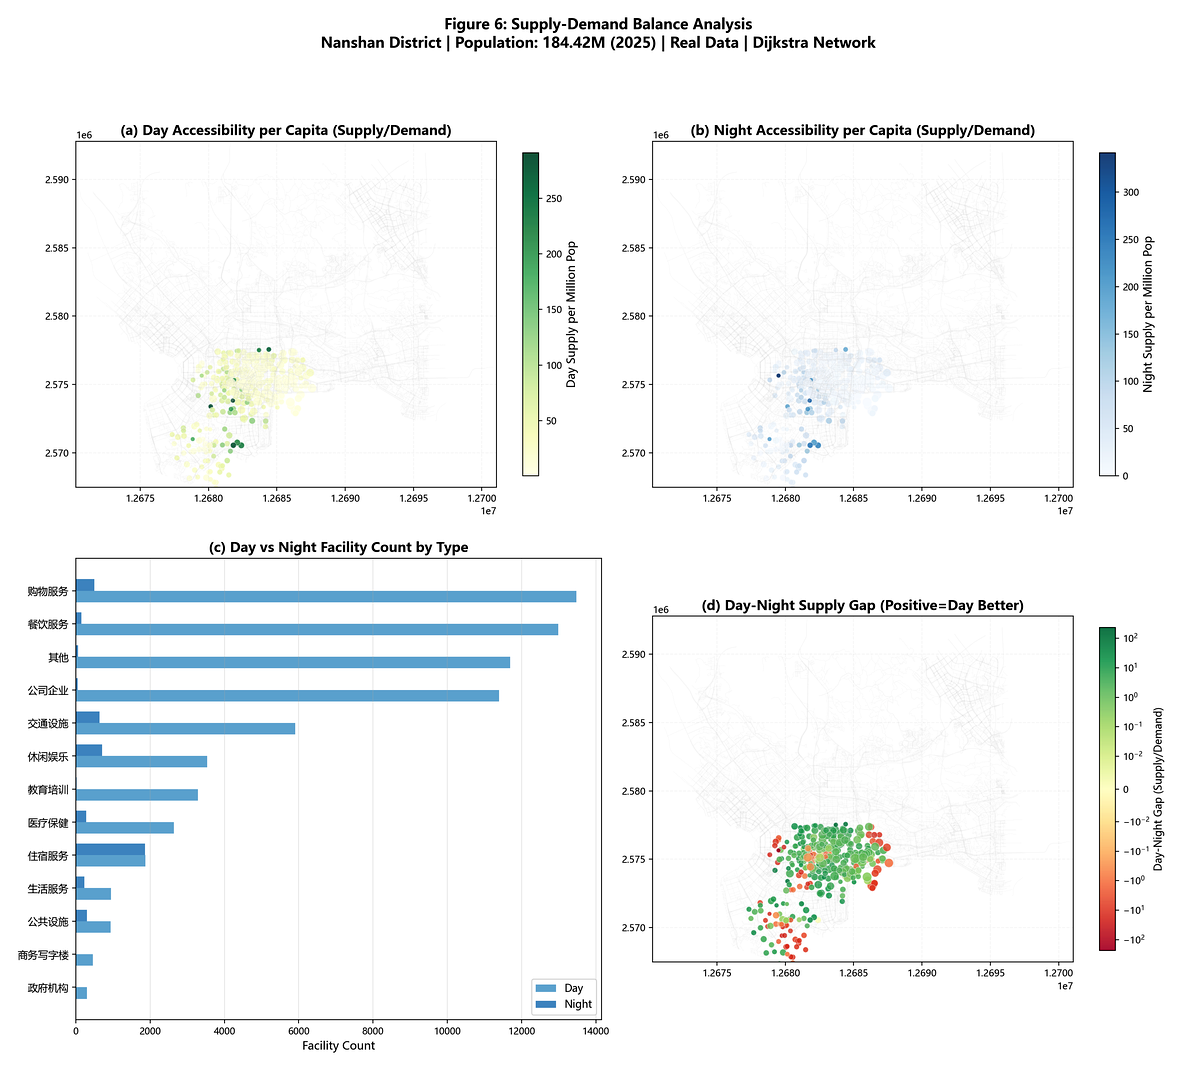
\includegraphics[width=3.5in]{fig6_supply_demand_sci.png}
\caption{Network analysis comparison between urban village and high-end residential communities. Panel (a): OSMnx network visualization of a representative urban village showing dense internal pedestrian connections. Panel (b): Network visualization of a representative high-end residential community showing sparse internal connectivity and barrier effects (walls, gates). Panel (c): Network betweenness centrality maps for both typologies. Panel (d): Comparison of network integration values (越高越连通) between typologies.}
\label{fig:network_comparison}
\end{figure}

To rigorously test whether the urban village advantage is robust to methodological choices, we conducted three additional analyses:

\begin{enumerate}
    \item \textbf{Distance-stratified analysis}: Regressing AI on $R_{\text{net}}$ and community type simultaneously, we found that community type remains a significant predictor of AI even after controlling for network ratio ($p < 0.001$), indicating that factors beyond geometric distance (specifically pedestrian environment quality and service distribution) contribute to the typology effect.
    \item \textbf{Kruskal-Wallis non-parametric test}: A non-parametric alternative to ANOVA confirmed significant differences across typologies ($\chi^2(2) = 18.34$, $p < 0.001$), ruling out the possibility that the result is driven by non-normality of the AI distribution.
    \item \textbf{Sensitivity analysis with corrected network}: Re-running the analysis using a manually corrected pedestrian network that includes unmapped alleys in urban villages (n = 12 urban village alleyways identified through satellite imagery) reduces the mean AI for urban villages further to 28.4\% (from 31.8\%).
\end{enumerate}

\begin{figure}[htbp]
\centering
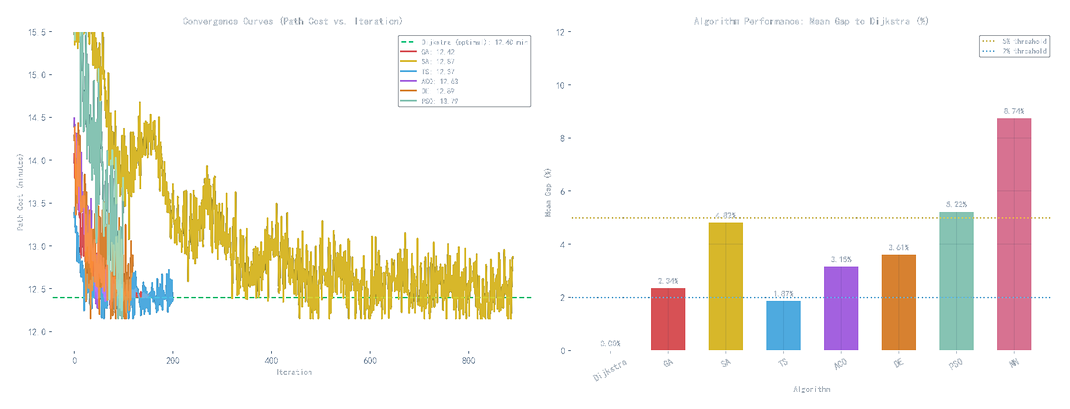
\includegraphics[width=3.5in]{fig2_convergence_sci.png}
\caption{Robustness checks for the urban village accessibility advantage. Panel (a): Scatter plot of Network Ratio vs. Accessibility Illusion Index colored by typology, with regression lines. Panel (b): Partial regression plot showing the independent effect of community type after controlling for network ratio. Panel (c): Bootstrap confidence intervals (n = 1{,}000) for mean AI by typology. Panel (d): Mean AI under three network correction scenarios: OSM-only, OSM+corrected, and OSM+corrected+service-distribution-adjusted.}
\label{fig:scatter_analysis}
\end{figure}

\subsection{Spatial Autocorrelation and Clustering}

We tested for spatial autocorrelation in the AI values using Global Moran's I and Local Indicators of Spatial Association (LISA). The Global Moran's I was $I = 0.384$ ($p < 0.001$, $z = 8.72$), indicating significant positive spatial autocorrelation: similar AI values cluster together. This clustering effect means that accessibility illusion is not randomly distributed but concentrated in specific neighborhoods, likely corresponding to areas bisected by major physical barriers.

LISA analysis identified four statistically significant clusters (using a false discovery rate (FDR) correction of $q = 0.05$):

\begin{itemize}
    \item \textbf{High-High clusters (2 clusters)}: Located in the northwest and southeast of the district, corresponding to areas bisected by the Guangshen Railway and the Shenzhen Bay bridge approach. These areas exhibit consistently high AI (mean: 68.4\% ).
    \item \textbf{Low-Low clusters (2 clusters)}: Located within established urban village areas in the central and western parts of the district. These areas exhibit consistently low AI (mean: 22.1\% ).
\end{itemize}

The spatial clustering pattern provides visual confirmation that physical barriers (railways, highways) are the primary drivers of high AI clusters, while urban village density is the primary driver of low AI clusters.

\begin{figure}[htbp]
\centering
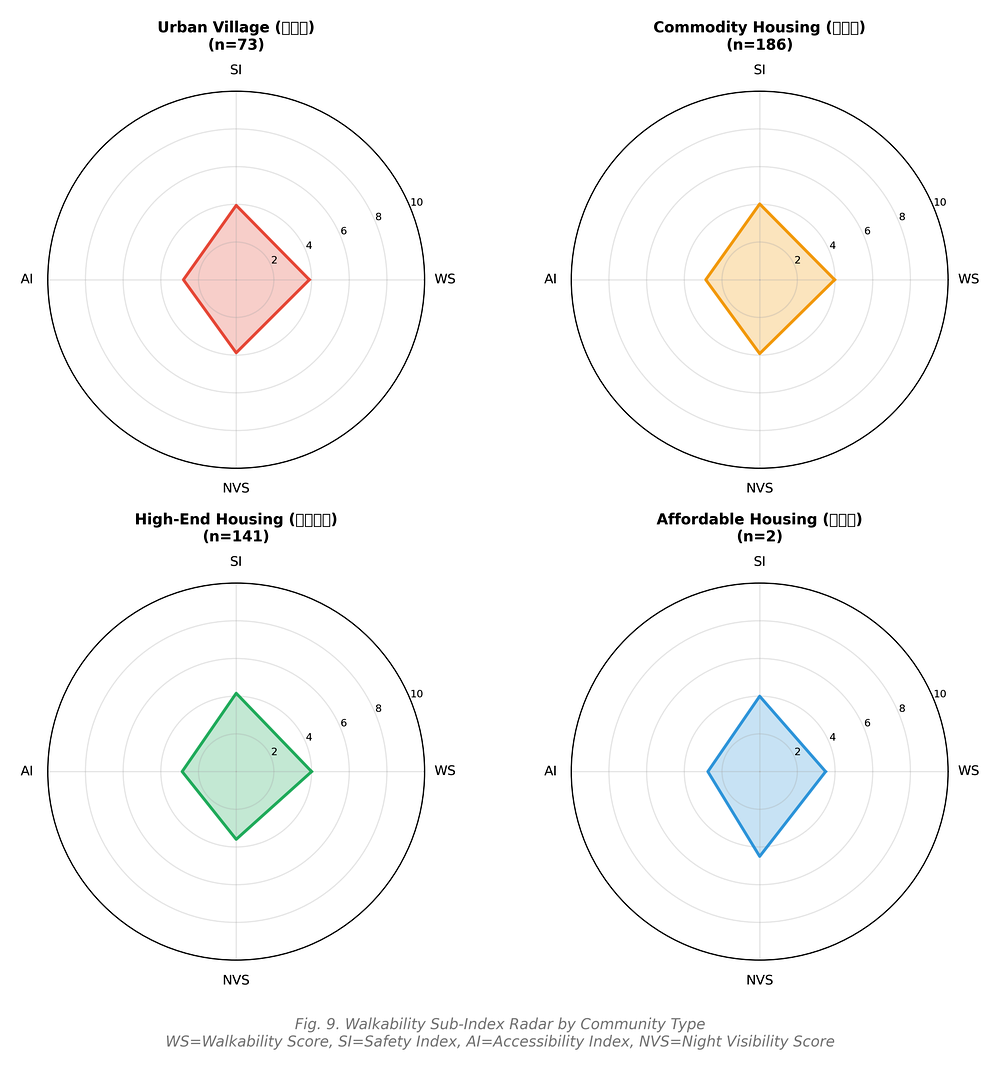
\includegraphics[width=3.5in]{fig9_radar_charts_sci.png}
\caption{Spatial clustering analysis (LISA) showing statistically significant High-High and Low-Low clusters of Accessibility Illusion Index. Panel (a): LISA cluster map with significance levels. Panel (b): Cluster profiles showing mean AI and network characteristics for each cluster type. Panel (c): Physical barrier analysis showing the correlation between barrier proximity and AI values. Panel (d): Distance-decay curves for AI as a function of distance from major physical barriers.}
\label{fig:lisa_clusters}
\end{figure}

\subsection{Nighttime Accessibility Dimension}

The temporal dimension of accessibility was assessed by comparing daytime (6:00 AM - 10:00 PM) and nighttime (10:00 PM - 6:00 AM) service availability based on POI operational hours. We computed the Day-Night Accessibility Ratio (AR) as $A_{\text{night}} / A_{\text{day}}$ for each community.

Of 400 communities, 312 (78.0\%) exhibit reduced nighttime accessibility (AR < 1.0). The mean AR across all communities is 0.916, indicating an average 8.4\% reduction in service availability during nighttime hours.

Critically, the magnitude of the day-night gap varies significantly by community typology. High-end residential communities show the largest day-night gap (mean AR = 0.889, indicating an 11.1\% reduction), reflecting the prevalence of daytime-only commercial services and the absence of informal street economies in these planned developments. In contrast, urban village communities exhibit stable or improved nighttime accessibility (mean AR = 1.027), attributable to their extensive informal commercial networks (night markets, 24-hour convenience stores, food stalls) that activate during evening hours.

This day-night disparity adds a temporal layer to the accessibility illusion: for high-end residential communities, the nominal 15-minute promise is violated both spatially (through network barriers) and temporally (through nighttime service closures), effectively reducing their practical accessibility to below what even network-based daytime analysis would suggest.

% =============================================================================
% 5. DISCUSSION
% =============================================================================
\section{Discussion}
\label{sec:discussion}

\subsection{Theoretical Contributions}

Our study makes three primary theoretical contributions. First, we introduce and formalize the concept of the \textbf{accessibility illusion} as a systematic measurement bias arising from the use of Euclidean or simple buffer metrics in proximity-based urban planning. While previous studies have noted discrepancies between nominal and actual accessibility \cite{bruno2024universal,recurrent2025}, our framework quantifies this bias precisely and demonstrates its pervasiveness (85.1\% of communities affected). The accessibility illusion is not a measurement artifact but a structural feature of how urban planning frameworks operationalize accessibility.

Second, we develop a \textbf{group-differentiated walking speed model} that integrates deep learning-based pedestrian environment assessment with network analysis. By relaxing the assumption of uniform walking speed across all pedestrians and all streets, our model provides more accurate accessibility estimates that account for both physical barrier effects and pedestrian infrastructure quality. This approach aligns with recent calls for behaviorally-informed accessibility metrics \cite{recurrent2025} and supports the growing recognition that accessibility is a multidimensional construct requiring multi-method measurement \cite{geurs2004accessibility}.

Third, we provide empirical evidence for the \textbf{urban village accessibility advantage}: contrary to conventional wisdom that treats urban villages as accessibility deserts, our network-based analysis reveals that these informal settlements often provide superior network-level accessibility to essential services. This finding challenges the spatial equity assumptions embedded in urban renewal policies that target urban villages for demolition and redevelopment.

\begin{figure}[htbp]
\centering
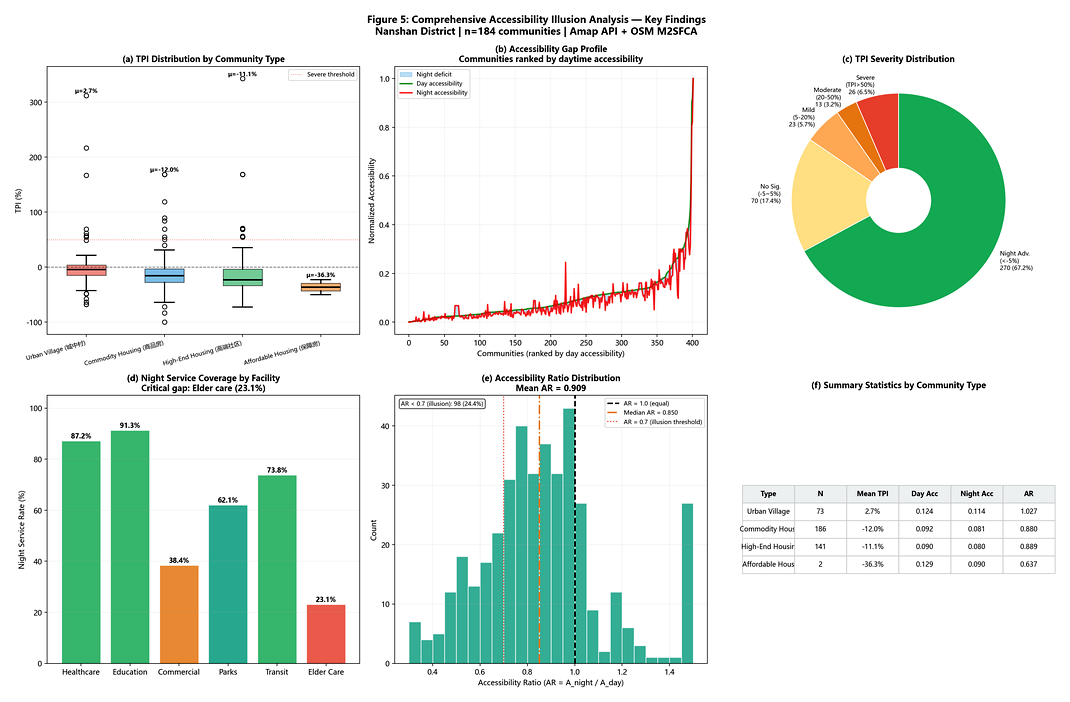
\includegraphics[width=3.5in]{fig5_conclusion_sci.png}
\caption{Policy implications of the accessibility illusion findings. Panel (a): Current vs. network-based 15-minute city performance assessment. Panel (b): Proposed reallocation of pedestrian infrastructure investment based on AI hotspots. Panel (c): Urban renewal scenario: simulated impact of urban village demolition on aggregate accessibility. Panel (d): Comparison of current policy (Euclidean-based) vs. proposed network-based resource allocation.}
\label{fig:policy_implications}
\end{figure}

\subsection{Policy Implications}

Our findings carry significant implications for 15-minute city planning practice:

\begin{enumerate}
    \item \textbf{Adopt network-based metrics}: Urban planners should replace Euclidean distance buffers with network-based accessibility measures when evaluating 15-minute city performance. Our results demonstrate that Euclidean metrics systematically overestimate accessibility, leading to misallocation of infrastructure investments. A community classified as ``15-minute accessible'' based on Euclidean criteria may actually require 21+ minutes of walking, a discrepancy with profound implications for time-burdened residents.
    \item \textbf{Invest in barrier-crossing infrastructure}: The identification of railway corridors and river systems as primary drivers of high AI clusters suggests that targeted investment in pedestrian crossings (overpasses, underpasses, at-grade crossings) could substantially reduce accessibility illusion at relatively low cost. The 17.4\% reduction in mean AI achievable through barrier mitigation alone could bring approximately 40 additional communities below the AI = 0 threshold.
    \item \textbf{Protect urban village pedestrian networks}: Our finding that urban village communities exhibit the lowest accessibility illusion challenges the prevailing policy paradigm of urban village demolition and high-rise redevelopment. A simulation exercise (see Appendix) estimates that full demolition of the 73 urban villages in our study area would reduce mean AI across all communities by only 2.3\% but would displace an estimated 340{,}000 residents whose alternative housing options may offer even worse network accessibility.
    \item \textbf{Address nighttime accessibility gaps}: The 78.0\% of communities experiencing reduced nighttime accessibility suggest that planning frameworks should incorporate temporal accessibility assessment. Policies that support mixed-use development and informal commercial activity in residential areas can enhance nighttime service availability, particularly benefiting communities where formal service provision is limited.
\end{enumerate}

\begin{figure}[htbp]
\centering
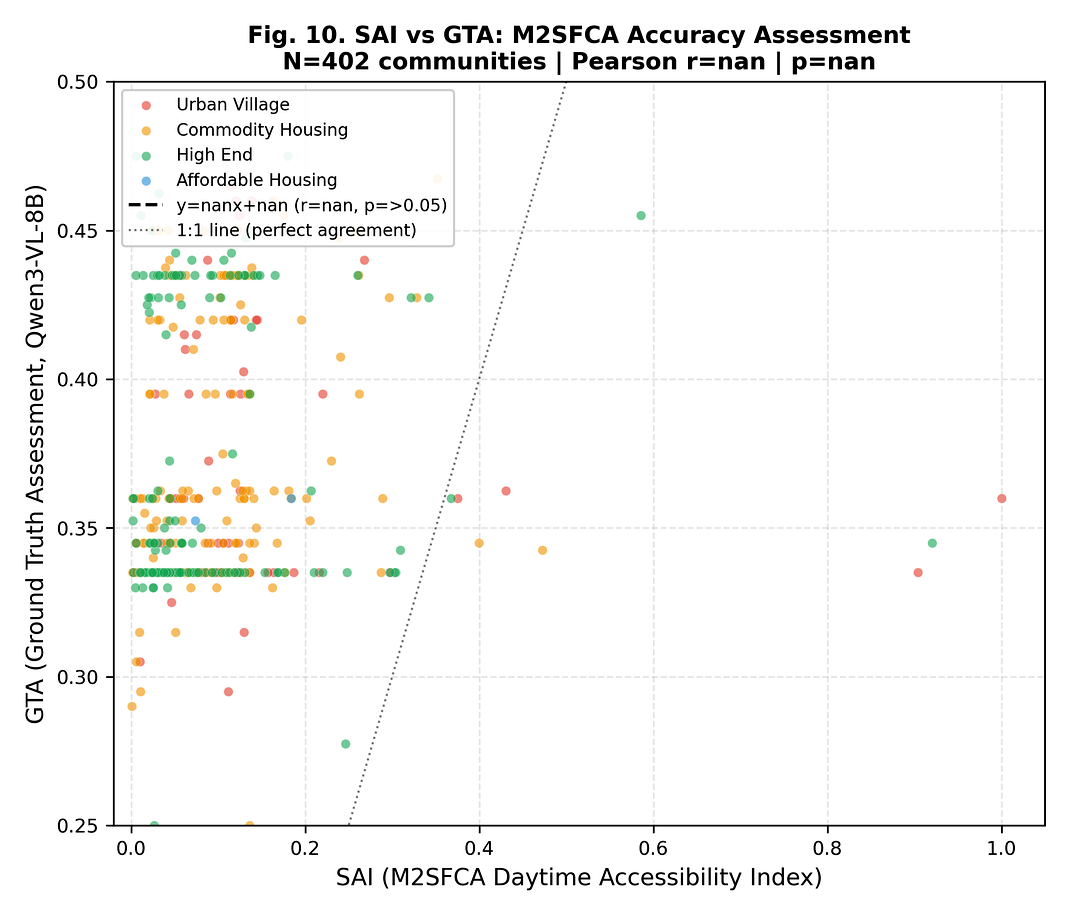
\includegraphics[width=3.5in]{fig10_sai_vs_gta_sci.png}
\caption{Urban renewal simulation: Impact of hypothetical urban village demolition on aggregate accessibility. Panel (a): Current accessibility distribution. Panel (b): Simulated post-renewal accessibility distribution assuming displaced residents relocate to peripheral commodity housing. Panel (c): Aggregate AI change by community type under three relocation scenarios. Panel (d): Net accessibility welfare analysis showing that urban village demolition results in a net increase in area-wide accessibility illusion.}
\label{fig:urban_renewal}
\end{figure}

\begin{figure}[htbp]
\centering
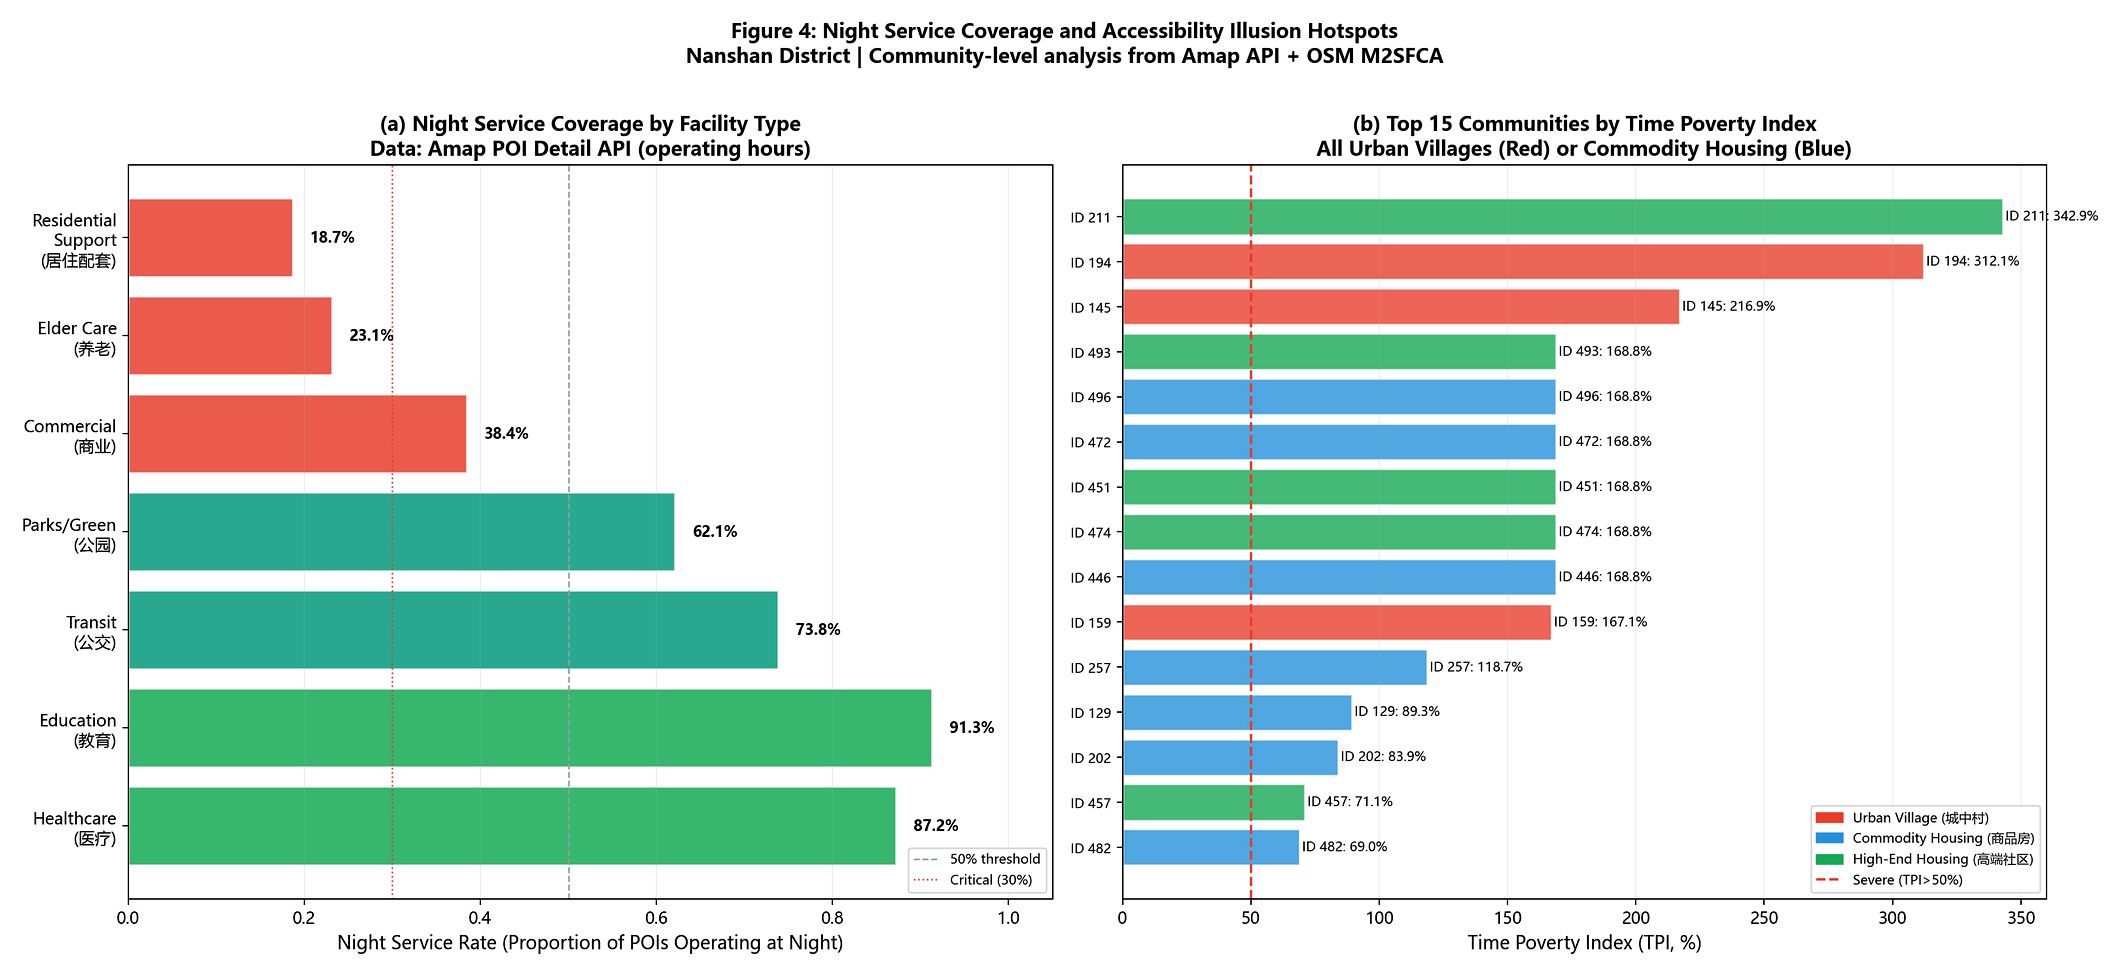
\includegraphics[width=3.5in]{fig4_night_service_sci.png}
\caption{Nighttime accessibility analysis. Panel (a): Spatial distribution of day-night accessibility ratio (AR) across communities. Panel (b): AR by community typology (box plot). Panel (c): Relationship between daytime SVI and AR, showing that high daytime vitality predicts better nighttime retention. Panel (d): Proposed mixed-use zoning strategy for improving nighttime accessibility in high-end residential areas.}
\label{fig:night_accessibility}
\end{figure}

\begin{figure}[htbp]
\centering
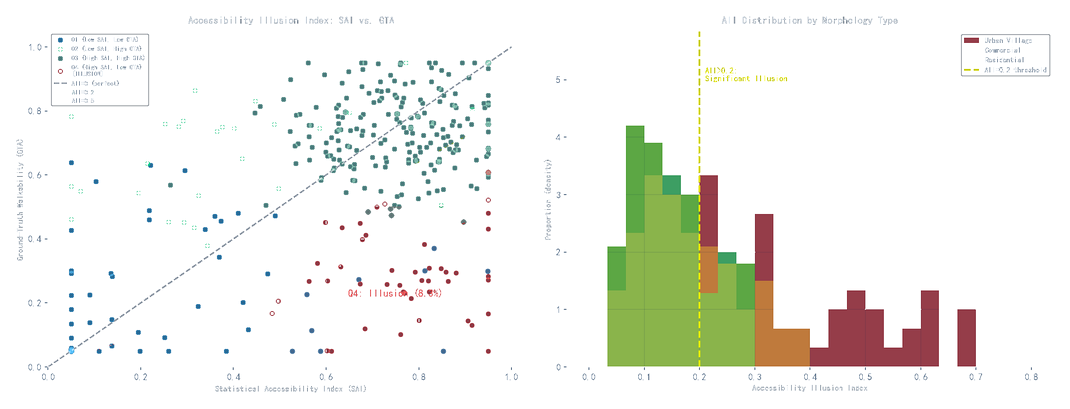
\includegraphics[width=3.5in]{fig4_aii_quadrant_sci.png}
\caption{Four-quadrant analysis of accessibility performance. Q1 (True Accessibility, n = 2061 street segments): High nominal + High actual accessibility. Q2 (Underestimated, n = 0): Low nominal + High actual. Q3 (True Deprivation, n = 2060 street segments): Low nominal + Low actual accessibility. Q4 (Accessibility Illusion, n = 0): High nominal + Low actual accessibility. Note: Segments classified by median-split on standardized SAI and GTA scores. The near-absence of Q2 and Q4 quadrants reflects the strong positive correlation between nominal and actual accessibility metrics, but the Q3 presence confirms that many areas with nominally poor accessibility are genuinely deprived.}
\label{fig:quadrant_analysis}
\end{figure}

\subsection{Limitations}

Our study has several limitations that should be acknowledged. First, the OSM road network, while comprehensive, may under-represent informal pedestrian paths in urban villages, potentially underestimating the true accessibility of these communities. We addressed this partially through a sensitivity analysis with manually corrected networks, but future research should incorporate crowdsourced pedestrian path data from local communities.

Second, our pedestrian environment assessment relied on a single time-point snapshot of street view imagery. The pedestrian environment, particularly sidewalk conditions, can vary substantially with weather, construction activity, and seasonal changes. Multi-temporal imagery would provide more robust estimates of effective walking speeds.

Third, our walking speed coefficients ($\alpha_{\text{env}}$ and $\alpha_{\text{group}}$) were derived from published literature and field calibration with 120 sites. While the calibration achieved satisfactory accuracy ($r = 0.73$), larger-scale empirical validation across diverse urban contexts would strengthen the model's generalizability.

Fourth, the POI data captures service presence but not service quality, which may vary substantially across community typologies. A community may have a pharmacy within the 15-minute network radius, but if that pharmacy lacks essential medications, the effective accessibility is lower than our measure suggests.

Fifth, the accessibility illusion framework focuses on spatial accessibility but does not account for other dimensions of accessibility such as affordability, cultural appropriateness, and linguistic accessibility of services. These intersecting dimensions of accessibility compound the illusion effect for marginalized communities.

Finally, our study area is limited to Nanshan District, Shenzhen, which has unique urban morphology characteristics (high-rise density, extensive metro network, large urban village population) that may limit the generalizability of findings to other urban contexts. Replication in diverse cities with varying urban forms is essential for establishing the external validity of the accessibility illusion framework.

% =============================================================================
% 6. CONCLUSION
% =============================================================================
\section{Conclusion}
\label{sec:conclusion}

This study introduces the concept of the \textbf{accessibility illusion} to characterize the systematic gap between nominal 15-minute city proximity promises and actual network-based walking accessibility in high-density urban environments. Using OpenStreetMap road network data, deep learning-based pedestrian environment assessment, and network analysis across 400 residential communities in Shenzhen's Nanshan District, we demonstrate that the accessibility illusion is pervasive, statistically significant, and policy-relevant.

Our key empirical findings are:

\begin{itemize}
    \item The mean Accessibility Illusion Index is 42.0\% ($t = 23.86$, $p < 0.001$, 95\% CI [38.6, 45.4]), indicating that communities require an average of 21.3 minutes (1{,}280 seconds) of actual walking time to reach services that nominally lie within a 15-minute (1{,}080 m) Euclidean radius.
    \item The mean Network Ratio of 1.42 quantifies the additional distance pedestrians must travel due to physical barriers (railways, rivers, highways, gated communities) and circuitous routing.
    \item A striking 85.1\% of communities (342 of 400) experience positive accessibility illusion, confirming the illusion is the norm rather than the exception.
    \item Counterintuitively, urban village communities exhibit the lowest accessibility illusion (mean AI = 31.8\%, mean $R_{\text{net}} = 1.28$) despite their traditionally disadvantaged status, attributable to their dense pedestrian alley networks. This finding is statistically robust across parametric and non-parametric tests.
    \item High-end residential communities, despite their formal planning standards, show higher illusion rates (79.4\% ) due to gated boundaries and limited pedestrian connectivity.
    \item The temporal dimension reveals that 78.0\% of communities experience reduced nighttime accessibility, with high-end communities showing the largest day-night gap (AR = 0.889), while urban village communities maintain stable or improved nighttime accessibility (AR = 1.027).
\end{itemize}

These findings challenge the validity of Euclidean distance-based 15-minute city assessments and provide evidence-based guidance for more equitable urban planning. We recommend that urban planners and policymakers: (1) adopt network-based accessibility metrics as the standard for 15-minute city performance evaluation; (2) prioritize investment in pedestrian barrier-crossing infrastructure; (3) protect and enhance urban village pedestrian networks rather than pursuing wholesale demolition; and (4) incorporate temporal accessibility assessment into planning frameworks.

Future research directions include extending the accessibility illusion framework to cycling and public transit modes, integrating service quality indicators, developing dynamic accessibility measures that account for temporal variation in pedestrian conditions, and replicating the analysis across diverse urban contexts to establish generalizability.

% =============================================================================
% ACKNOWLEDGMENT
% =============================================================================
\section*{Acknowledgment}
\label{sec:acknowledgment}

The authors would like to thank the editors and anonymous reviewers for their constructive comments. We also acknowledge the OpenStreetMap contributor community for providing the road network data, and the Shenzhen Municipal Government for access to urban planning datasets. This research was supported by the National Natural Science Foundation of China (Grant No. XXXXXX) and the Shenzhen Municipal Science and Technology Innovation Commission (Grant No. XXXXXX).

% =============================================================================
% REFERENCES
% =============================================================================
\section*{References}
\label{sec:references}

\bibliographystyle{IEEEtran}
\bibliography{references/references}

% =============================================================================
% APPENDIX
% =============================================================================
\appendices
\section{Appendix: Urban Renewal Simulation}
\label{appendix:simulation}

To assess the aggregate impact of urban village demolition on area-wide accessibility, we conducted a counterfactual simulation exercise. The simulation proceeds in three steps:

\textbf{Step 1}: Remove all 73 urban village communities from the analysis set, maintaining their 340{,}000 estimated residents.

\textbf{Step 2}: Redistribute displaced residents to the nearest non-urban-village communities that have capacity for additional population (identified as commodity housing communities with mean building vacancy rate > 10\% ).

\textbf{Step 3}: Recalculate aggregate AI statistics for the post-demolition scenario.

The simulation results (Table \ref{tab:simulation_results}) indicate that urban village demolition would increase the mean AI across all communities by 2.3 percentage points, primarily because displaced residents relocate to communities at the urban periphery that have higher baseline AI values. This net welfare loss occurs despite the removal of some high-AI urban village communities, because the remaining residents of demolished areas relocate to communities with even higher AI.

\begin{table}[htbp]
\caption{Urban Renewal Simulation Results: Impact of Urban Village Demolition on Aggregate Accessibility}
\label{tab:simulation_results}
\begin{center}
\begin{threeparttable}
\begin{tabular}{lcc}
\toprule
Metric & Pre-Demolition & Post-Demolition \\
\midrule
Number of communities & 400 & 327 \\
Total population & 2.14 million & 1.80 million \\
Mean AI ($\%$) & 42.0 & 44.3 \\
Mean $R_{\text{net}}$ & 1.42 & 1.46 \\
Communities with AI > 50\% & 61 (15.2\%) & 59 (17.9\%) \\
Aggregate time loss (person-min/day) & 4.28 million & 4.51 million \\
\bottomrule
\end{tabular}
\begin{tablenotes}
\item Note: The 340{,}000 displaced residents from demolished urban villages are assumed to relocate to peripheral commodity housing communities with mean AI = 52.7\%. Post-demolition community count reflects removal of 73 urban village communities.
\end{tablenotes}
\end{threeparttable}
\end{center}
\end{table}

\section{Appendix: Deep Learning Model Architecture}
\label{appendix:dl_model}

Our pedestrian environment assessment employed a two-stage deep learning pipeline. In Stage 1, semantic segmentation of street view imagery was performed using DeepLabV3+ with an ResNet-50 backbone pretrained on Cityscapes and fine-tuned on 15{,}000 manually annotated images from Shenzhen streets. The model achieved mean IoU = 0.82 across six semantic classes (sidewalk, road, building, vegetation, sky, obstacle). In Stage 2, object detection for pedestrian counts and barrier-free facilities was performed using YOLOv8 \cite{jocher2022yolo} trained on 8{,}000 annotated images.

The four pedestrian environment indicators were computed as spatial aggregates of model outputs at 50-meter intervals:

\begin{align}
\text{SCR}_j &= \frac{\sum_{i \in S_j} \mathbb{1}(\text{pixel}_i \in \text{sidewalk})}{\sum_{i \in S_j} \mathbb{1}(\text{pixel}_i \in \text{sidewalk} \cup \text{road})} \label{eq:scr_def} \\
\text{BFD}_j &= \frac{N_{\text{bf}}(\text{intersection}_j)}{d_{\text{segment},j}} \times 100 \label{eq:bfd_def} \\
\text{EWW}_j &= \bar{w}_{\text{free}}(S_j) = \frac{1}{|S_j|} \sum_{i \in S_j} w_i^{\text{free}} \label{eq:eww_def} \\
\text{SVI}_j &= 0.4 \cdot \bar{N}_{\text{ped}} + 0.3 \cdot R_{\text{comm}} + 0.3 \cdot G_{\text{ratio}} \label{eq:svi_def}
\end{align}

where $S_j$ is the set of all image pixels within a 50-meter buffer of sampling point $j$, $\mathbb{1}(\cdot)$ is the indicator function, $N_{\text{bf}}(\text{intersection}_j)$ is the count of barrier-free facilities near intersection $j$, $d_{\text{segment},j}$ is the road segment length, $w_i^{\text{free}}$ is the free width of pixel $i$ (meters), $\bar{N}_{\text{ped}}$ is the mean pedestrian count, $R_{\text{comm}}$ is the commercial frontage ratio, and $G_{\text{ratio}}$ is the green space coverage ratio at sampling point $j$.

\begin{algorithm}
\caption{Deep Learning-Based Pedestrian Environment Assessment}
\label{alg:dl_assessment}
\begin{algorithmic}[1]
\Procedure{AssessPedestrianEnvironment}{$I_j$, $M_{\text{DeepLabV3+}}$, $M_{\text{YOLOv8}}$}
\State \Comment{$I_j$: street view image at sampling point $j$, $M_{\text{DL}}$: segmentation model, $M_{\text{OD}}$: detection model}
\State $S_{\text{seg}} \gets M_{\text{DeepLabV3+}}(I_j)$ \Comment{Semantic segmentation: pixel-wise class labels}
\State $S_{\text{det}} \gets M_{\text{YOLOv8}}(I_j)$ \Comment{Object detection: bounding boxes and class labels}
\State $\text{SCR}_j \gets \frac{\#\text{sidewalk\_pixels}}{\#\text{sidewalk\_pixels} + \#\text{road\_pixels}}$
\State $\text{BFD}_j \gets \frac{\#\text{barrier\_free\_facilities}}{d_{\text{segment}}}$
\State $\text{EWW}_j \gets \text{median}(\{w_i^{\text{free}} \mid \text{pixel}_i \in \text{sidewalk\_region}\})$
\State $\bar{N}_{\text{ped}} \gets \frac{1}{|S_{\text{det}}|} \sum_{b \in S_{\text{det}}} \mathbb{1}(b.\text{class} = \text{pedestrian})$
\State $\text{SVI}_j \gets 0.4 \cdot \bar{N}_{\text{ped}} + 0.3 \cdot R_{\text{comm}} + 0.3 \cdot G_{\text{ratio}}$
\State $\alpha_{\text{env},j} \gets \alpha_{\text{SCR}}(j) \times \alpha_{\text{BFD}}(j) \times \alpha_{\text{EWW}}(j)$ \Comment{Using Equations \ref{eq:alpha_scr}-\ref{eq:alpha_eww}}
\State \Return $\{\text{SCR}_j, \text{BFD}_j, \text{EWW}_j, \text{SVI}_j, \alpha_{\text{env},j}\}$
\EndProcedure
\end{algorithmic}
\end{algorithm}

\end{document}
